\documentclass[11pt]{article}

\usepackage[margin=1in]{geometry}
\usepackage{amsmath,amssymb}
\usepackage{graphicx}
\usepackage{booktabs}
\usepackage{array}
\usepackage{longtable}
\usepackage{siunitx}
\usepackage{tikz}
\usetikzlibrary{arrows.meta,positioning,fit,backgrounds}
\usepackage[hidelinks]{hyperref}

\newcommand{\thenote}{\emph{Booster Landing: Two Solution Routes, Five
Certification Gates}}
\newcommand{\noteS}[1]{\thenote, \S#1}
\newcommand{\Tmin}{T_{\min}}
\newcommand{\Tmax}{T_{\max}}
\newcommand{\etaT}{\eta_T}
\newcommand{\file}[1]{\texttt{#1}}

% Compact description-style column types used by the module tables.
\newcolumntype{L}[1]{>{\raggedright\arraybackslash}p{#1}}

\title{Software Description Document:\\
The \texttt{booster\_landing} Powered-Descent Guidance Campaign}

\author{Michael Casey}

\date{9 August 2026}

% Long \texttt{} identifiers are unbreakable; let TeX stretch rather than
% overflow the margin.
\sloppy
\setlength{\emergencystretch}{3em}

\begin{document}
\maketitle

\begin{center}
\fbox{\parbox{0.86\textwidth}{\small\textbf{As-built stamp.} This document
describes the campaign at commit \texttt{77bf8e9} (2026-08-09), against the
shipped \file{results/booster\_run.mat} of \textbf{09-Aug-2026 12:56:25} ---
a full \texttt{cfg.phase2 = true} run, so the file carries the complete
schema of \S\ref{sec:data}. Every measured number quoted below was read
from that artifact or from the source at that commit. \emph{Refresh trigger:}
re-stamp this box, and re-check \S\ref{sec:data}'s variable list and the
flagship numbers in \S\ref{sec:tests:flagship}, after any run that replaces
\file{booster\_run.mat}.}}
\end{center}

\vspace{0.6em}

\begin{abstract}
This is the software-as-built description of the \file{booster\_landing}
campaign: a 3-DOF minimum-fuel powered-descent guidance (PDG) problem solved
two independent ways, certified by a five-gate layer, closed with a
time-varying LQR tracker, and Monte-Carlo tested under dispersions. It
documents architecture, every module's calling interface field by field,
data flow, on-disk schemas, the certification and test architectures, the
coding conventions the campaign holds itself to, and its extension points
and known limitations. It is the companion to two other documents in this
repository, and deliberately does not duplicate either: the theory note
\thenote{} (\file{doc/booster\_landing\_note.tex}) derives the mathematics
and reports the measured results, and \file{README.md} says how to run the
thing. This document says what the software \emph{is}, for an engineer who
must extend or audit it without the session history that produced it. Every
interface below was transcribed from the source; where the source's own
comments and the README disagree, the code is documented and the
disagreement is flagged (\S\ref{sec:discrepancies}).
\end{abstract}

\tableofcontents

%==============================================================
\section{System overview}
\label{sec:overview}

\subsection{Purpose}

The campaign answers one engineering question --- \emph{can a Falcon-9-class
booster land on the pad, and can we prove it} --- with a deliberately
redundant software structure. The min-fuel PDG problem is posed once and
solved twice by methods that share no solver formulation (only the
parameter set and the dynamics model): a free-final-time Hermite--Simpson
collocation NLP that carries the nonconvex thrust annulus directly, and a
lossless convexification solved as fixed-time convex subproblems under a
golden-section search on $t_f$. A certification layer then scores the pair
against five substantive gates G1--G5, plus a time-base gate G0 that
certifies the basis the other five are computed on. Only after certification does the guidance solution feed
the tracking half of the pipeline: a phase-scheduled time-varying LQR, a
dispersed closed-loop truth simulation, and a Monte-Carlo campaign.

The redundancy is the point. Route A and Route B are the cross-check
(gate~G3); the gates are the check on \emph{each} route individually; and
the closed-loop simulation is the check that the certified trajectory is
flyable rather than merely optimal.

\subsection{Two phases}

\textbf{Phase 1 (vacuum)} is the certified, flagship configuration.
Convexification is exactly valid in vacuum, so Route B exists and gates
G3/G4 are live. This is what a no-argument \file{run\_booster\_landing} run
produces.

\textbf{Phase 2 (exponential atmosphere with drag)} is opt-in
(\texttt{cfg.phase2}) and is a \emph{comparison campaign layered on top of}
Phase 1, never a replacement. It re-solves Route A with
\texttt{P.drag.on = true}, warm-started from the Phase-1 vacuum solution,
and runs the same tracking/MC stack against it. There is no convex twin for
the drag problem, so \texttt{certify\_pdg} is called with an empty
\texttt{solV} and G3/G4 report \texttt{'skipped'}. Every other gate,
including G5's primer sub-check, applies to Phase 2 on exactly the same
terms as Phase 1 --- the $10^\circ$ drag primer loosening this campaign
once carried was withdrawn on 2026-08-09 when its cause turned out to be a
bug in the gate (\S\ref{sec:certify}). See
\noteS{Phase 2} for the physics and \S\ref{sec:certify} here for the
software semantics.

\subsection{Pipeline}

Figure~\ref{fig:arch} is the data flow. The front door
\file{run\_booster\_landing.m} executes the stages in order, printing a
\texttt{[k/5]} banner per stage, with Phase 2 appended as a sixth
(\texttt{[P2 +1]}) stage when requested.

\begin{figure}[htbp]
\centering
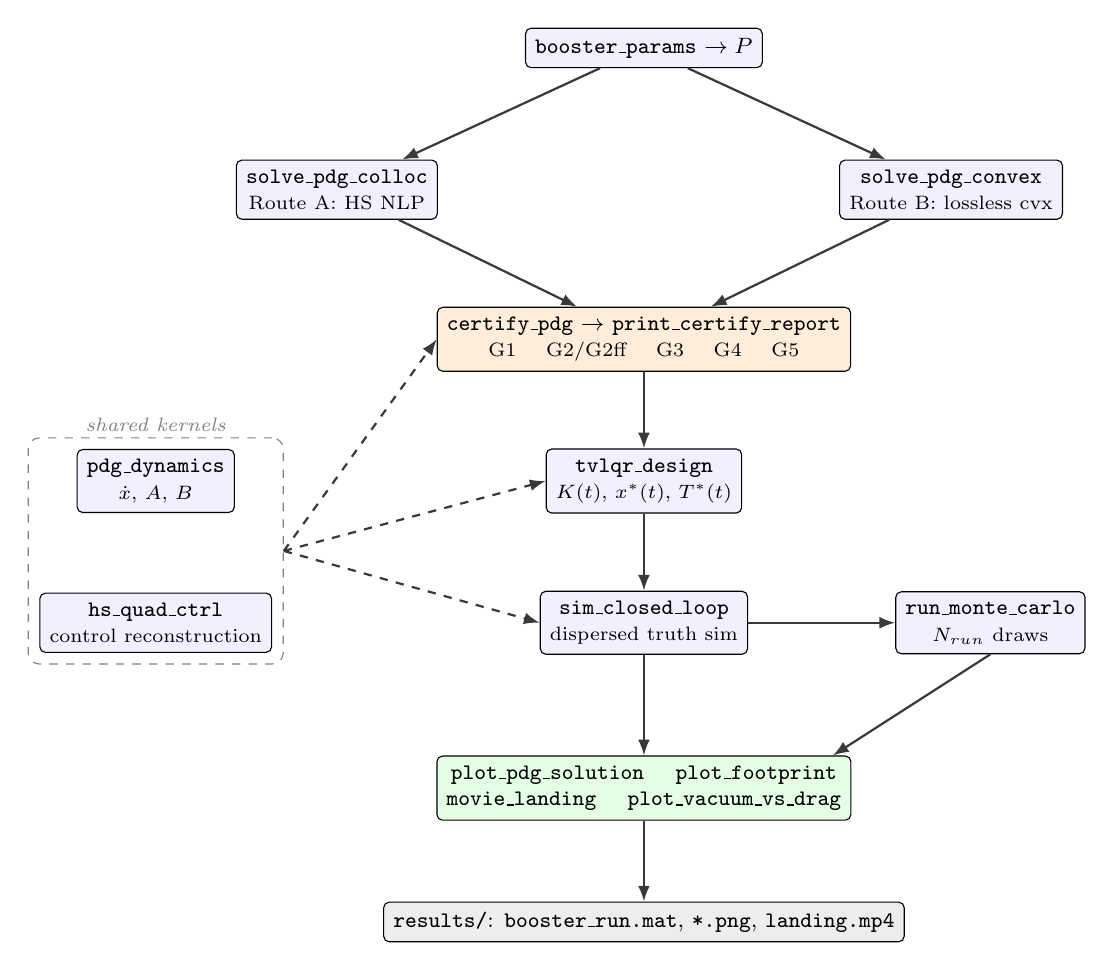
\begin{tikzpicture}[
  x=1cm, y=1cm,
  box/.style={draw, rounded corners=2pt, align=center, font=\footnotesize,
              inner sep=3.5pt},
  lib/.style={box, fill=blue!6},
  cert/.style={box, fill=orange!14},
  vizb/.style={box, fill=green!10},
  prod/.style={box, fill=gray!14},
  ar/.style={-{Latex[length=2mm]}, thick, gray!45!black},
  dar/.style={ar, dashed}
]

\node[lib] (params) at (0,0)
  {\texttt{booster\_params} $\rightarrow P$};
\node[lib] (colloc) at (-3.9,-1.8)
  {\texttt{solve\_pdg\_colloc}\\\scriptsize Route A: HS NLP};
\node[lib] (convex) at ( 3.9,-1.8)
  {\texttt{solve\_pdg\_convex}\\\scriptsize Route B: lossless cvx};
\node[cert] (certify) at (0,-3.7)
  {\texttt{certify\_pdg} $\rightarrow$ \texttt{print\_certify\_report}\\
   \scriptsize G1 \quad G2/G2ff \quad G3 \quad G4 \quad G5};
\node[lib] (tvlqr) at (0,-5.5)
  {\texttt{tvlqr\_design}\\\scriptsize $K(t)$, $x^*(t)$, $T^*(t)$};
\node[lib] (sim) at (0,-7.3)
  {\texttt{sim\_closed\_loop}\\\scriptsize dispersed truth sim};
\node[lib] (mc) at (4.4,-7.3)
  {\texttt{run\_monte\_carlo}\\\scriptsize $N_{run}$ draws};
\node[vizb] (vizn) at (0,-9.4)
  {\texttt{plot\_pdg\_solution} \quad \texttt{plot\_footprint}\\
   \texttt{movie\_landing} \quad \texttt{plot\_vacuum\_vs\_drag}};
\node[prod] (out) at (0,-11.1)
  {\texttt{results/}: \texttt{booster\_run.mat}, \texttt{*.png},
   \texttt{landing.mp4}};

\node[lib] (dyn) at (-6.2,-5.5)
  {\texttt{pdg\_dynamics}\\\scriptsize $\dot x$, $A$, $B$};
\node[lib] (hs) at (-6.2,-7.3)
  {\texttt{hs\_quad\_ctrl}\\\scriptsize control reconstruction};
\node[draw, dashed, gray, rounded corners, fit=(dyn)(hs), inner sep=4pt,
      label={[font=\scriptsize\itshape, gray, inner sep=2pt]above:shared kernels}]
      (kern) {};

\draw[ar] (params) -- (colloc);
\draw[ar] (params) -- (convex);
\draw[ar] (colloc) -- (certify);
\draw[ar] (convex) -- (certify);
\draw[ar] (certify) -- (tvlqr);
\draw[ar] (tvlqr) -- (sim);
\draw[ar] (sim) -- (mc);
\draw[ar] (sim) -- (vizn);
\draw[ar] (mc.south) -- ([xshift=24mm]vizn.north);
\draw[ar] (vizn) -- (out);
\draw[dar] (kern.east) -- (certify.west);
\draw[dar] (kern.east) -- (tvlqr.west);
\draw[dar] (kern.east) -- (sim.west);

\end{tikzpicture}
\caption{Campaign architecture. Solid arrows are the stage sequence
\file{run\_booster\_landing.m} drives; dashed arrows are the two shared
kernels (\texttt{pdg\_dynamics} and \texttt{hs\_quad\_ctrl}) that
certification, tracking and simulation all call, which is what makes the
gates certify the control the tracker actually flies. Blue = \file{lib/},
orange = \file{certify/}, green = \file{viz/}. Route B and gates G3/G4 are
absent on the Phase-2 (drag) path.}
\label{fig:arch}
\end{figure}

\subsection{Repository layout}

\begin{center}
\begin{tabular}{@{}lL{10.4cm}@{}}
\toprule
Path & Contents \\
\midrule
\file{run\_booster\_landing.m} & Front door (the only script a user runs) \\
\file{setup\_paths.m} & Path bootstrap: campaign dirs + CasADi 3.7 \\
\file{lib/} & Parameters, dynamics, both solvers, control reconstruction,
tracker, truth sim, Monte Carlo (8 files) \\
\file{certify/} & Gate evaluation and gate-table printing (2 files) \\
\file{viz/} & Three static figures and one movie (4 files) \\
\file{tests/} & One \texttt{test\_*.m} per unit, plus the end-to-end
front-door contract test (11 files) \\
\file{doc/} & Theory note, this SDD, committed copies of the figures \\
\file{results/} & Generated products; git-ignored except \file{.gitkeep} \\
\file{process/} & Campaign ledger, per-task briefs and reports (history,
not interface) \\
\bottomrule
\end{tabular}
\end{center}

Sixteen \texttt{.m} files ship as production modules --- 1 front door,
1 path bootstrap, 8 library, 2 certification, 4 visualization --- plus the
11 test scripts, \textbf{27 \texttt{.m} files in all}.

\subsection{Execution model}

Every entry point is a MATLAB \emph{function} except the tests, which are
\emph{scripts}. That distinction is load-bearing --- see
\S\ref{sec:tests:runner}.

\file{run\_booster\_landing} calls \file{setup\_paths} as its first
statement, so a cold MATLAB needs nothing but a \texttt{cd} into the
campaign folder. \file{setup\_paths} resolves its own location via
\texttt{fileparts(mfilename('fullpath'))} and adds the campaign root,
\file{lib}, \file{certify}, \file{viz}, \file{tests}, and
\verb|$HOME/casadi-3.7.0|. Tests bootstrap themselves the same way
(\S\ref{sec:tests}).

The two solvers are the only modules with an external dependency: CasADi's
\texttt{Opti} interface driving IPOPT. Everything downstream --- gates,
Riccati integration, truth simulation, Monte Carlo, plots --- is plain
MATLAB plus \texttt{ode45}.

%==============================================================
\section{Parameter system}
\label{sec:params}

\subsection{\texttt{booster\_params()} fields}

\file{lib/booster\_params.m} is the single source of truth. It takes no
arguments and returns one struct. Nothing else in the campaign hardcodes a
physical constant.

\begin{center}
\begin{longtable}{@{}llL{7.0cm}@{}}
\toprule
Field & Value & Meaning / notes \\
\midrule
\endfirsthead
\toprule
Field & Value & Meaning / notes \\
\midrule
\endhead
\multicolumn{3}{@{}l}{\textit{Vehicle}}\\
\texttt{P.mdry} & \num{25600} & dry mass [kg] \\
\texttt{P.m0}   & \num{30000} & mass at landing-burn start [kg] \\
\texttt{P.Tmax} & \num{845e3} & one Merlin 1D, sea level [N] \\
\texttt{P.Tmin} & \texttt{0.40*P.Tmax} & \textbf{DERIVED} from
  \texttt{P.Tmax}; minimum throttle [N] \\
\texttt{P.etaT} & \num{0.87} & guidance thrust de-rate [--] (adjudicated;
  \S\ref{sec:params:adj}) \\
\texttt{P.Isp}  & \num{282} & sea-level specific impulse [s] \\
\texttt{P.g0}   & \num{9.80665} & standard gravity [m/s$^2$] \\
\texttt{P.gvec} & \texttt{[0;0;-P.g0]} & \textbf{DERIVED} from
  \texttt{P.g0}; flat-Earth gravity, $z$ up [m/s$^2$] \\
\midrule
\multicolumn{3}{@{}l}{\textit{Boundary conditions}}\\
\texttt{P.r0} & \texttt{[500;100;2000]} & post-entry-burn position [m] \\
\texttt{P.v0} & \texttt{[-30;0;-180]} & entry velocity [m/s] \\
\texttt{P.vf} & \texttt{[0;0;-1.5]} & terminal velocity target [m/s]
  (adjudicated; \S\ref{sec:params:adj}) \\
\midrule
\multicolumn{3}{@{}l}{\textit{Path constraints}}\\
\texttt{P.gs\_deg} & \num{30} & glideslope minimum elevation [deg] \\
\texttt{P.theta\_max\_deg} & \texttt{Inf} & thrust-pointing cone half-angle;
  \texttt{Inf} disables the constraint in both solvers
  (\S\ref{sec:extend:cone}) \\
\midrule
\multicolumn{3}{@{}l}{\textit{Discretization / solver}}\\
\texttt{P.N} & \num{60} & Hermite--Simpson segments (Route A) \\
\texttt{P.Nconv} & \num{120} & trapezoid nodes (Route B) \\
\texttt{P.tf\_lo} & \num{10} & free-final-time bracket lower bound [s] \\
\texttt{P.tf\_hi} & \num{22} & upper bound [s]; also sets Route A's
  nondimensional time scale $T_c=(t_{f,lo}+t_{f,hi})/2$. Validated in
  \emph{vacuum only} \\
\midrule
\multicolumn{3}{@{}l}{\textit{Atmosphere (Phase 2; off by default)}}\\
\texttt{P.drag.on}   & \texttt{false} & master switch, read by
  \texttt{pdg\_dynamics}, both solvers, \texttt{certify\_pdg},
  \texttt{sim\_closed\_loop}, \texttt{run\_monte\_carlo} \\
\texttt{P.drag.rho0} & \num{1.225} & sea-level density [kg/m$^3$] \\
\texttt{P.drag.H}    & \num{8500}  & scale height [m] \\
\texttt{P.drag.Cd}   & \num{1.0}   & drag coefficient [--] \\
\texttt{P.drag.A}    & \num{10.75} & reference area [m$^2$] \\
\midrule
\multicolumn{3}{@{}l}{\textit{Success criteria / Monte Carlo}}\\
\texttt{P.pad\_radius} & \num{15}  & landing accuracy requirement [m] \\
\texttt{P.vtd\_max}    & \num{2.0} & maximum touchdown speed [m/s] \\
\texttt{P.seed}        & \num{42}  & \texttt{rng} seed for all random draws \\
\bottomrule
\end{longtable}
\end{center}

One retired field is documented in the file but not set:
\texttt{P.zTermBand} (a 150\,m terminal-phase altitude gate) was removed
when \texttt{sim\_closed\_loop} moved to altitude-indexed guidance, which
makes the altitude-error channel identically zero everywhere and leaves
nothing for a band to gate. Nothing references it.

\subsection{The \texttt{cfg.P} override contract}
\label{sec:params:cfg}

The campaign's standing rule is that \emph{no parameter is ever changed by
editing a file}. \file{run\_booster\_landing} accepts an optional
\texttt{cfg} struct whose \texttt{cfg.P} sub-struct is merged onto
\texttt{booster\_params()} \textbf{field by field}:

\begin{verbatim}
P = booster_params();
if isfield(cfg, 'P')
    pf = fieldnames(cfg.P);
    for k = 1:numel(pf), P.(pf{k}) = cfg.P.(pf{k}); end
    ...
end
\end{verbatim}

This is a flat overwrite, which by itself would desynchronize the two
\textbf{derived} pairs marked in the table above. The front door therefore
re-derives a dependent whenever its parent was overridden and the dependent
was \emph{not} also given explicitly:

\begin{center}
\begin{tabular}{@{}lll@{}}
\toprule
Parent overridden & Dependent re-derived & Suppressed by \\
\midrule
\texttt{cfg.P.Tmax} & \texttt{P.Tmin = 0.40*P.Tmax} &
  supplying \texttt{cfg.P.Tmin} \\
\texttt{cfg.P.g0}   & \texttt{P.gvec = [0;0;-P.g0]} &
  supplying \texttt{cfg.P.gvec} \\
\bottomrule
\end{tabular}
\end{center}

An explicit dependent override always wins. When a re-derivation fires the
front door prints a \texttt{[cfg.P] ... re-derived ...} line, so the console
log is self-describing. \textbf{Invariant to preserve:} this covers exactly
the two parent/dependent pairs that exist today. Any new derived field added
to \file{booster\_params.m} must be added to this block as well, or a
\texttt{cfg.P} override of its parent will silently ship an inconsistent
parameter set that \texttt{certify\_pdg} will certify without complaint ---
gates check physics, not parameter-set self-consistency. An override of any
field \emph{not} documented as derived is a plain, unchecked overwrite.

\subsection{The four adjudicated values}
\label{sec:params:adj}

Four numbers in this campaign were set by explicit user adjudication after a
measurement, not by a default. Each is documented at length at its point of
definition. The design specification
(\file{docs/superpowers/specs/2026-08-08-booster-landing-design.md}) is the
designated tiebreaker if any restatement of these numbers --- here, in the
README, or in a source comment --- ever disagrees.

\begin{center}
\begin{longtable}{@{}lL{4.2cm}L{6.3cm}@{}}
\toprule
Value & Defined in & Substance \\
\midrule
\endfirsthead
\toprule
Value & Defined in & Substance \\
\midrule
\endhead
\texttt{P.etaT = 0.87} & \file{lib/booster\_params.m} &
Guidance solves against $\etaT\Tmax = 735.15$\,kN; the tracker and truth sim
keep the full $[\Tmin,\Tmax]$ annulus, so the 13\% is reserved feedback
headroom, not lost capability. Costs $+82.3$\,kg ($\approx1.9\%$) of
propellant. An earlier 0.93 shipped briefly and was measured insufficient.
See \noteS{The guidance thrust de-rate}. \\
\texttt{P.vf = [0;0;-1.5]} m/s & \file{lib/booster\_params.m} &
With $\Tmin$ exceeding vehicle weight at every mass, $v(t_f)=0$ at $z=0$ is
a singular endpoint: the closed loop arrests above the pad instead of
touching down. A small legs-absorbed descent rate (inside the
\texttt{P.vtd\_max}=2.0\,m/s gate) makes a genuine touchdown achievable.
See \noteS{The singular terminal boundary condition}. \\
G3 $|\Delta m_f| < 1.0$\,kg & \file{certify/certify\_pdg.m} &
Reclassified from an agreement tolerance (0.1\,kg) to a \emph{measurement}
threshold over the convex route's Taylor mass-bound model error. Measured
mid-campaign: \textbf{$0.70$--$0.94$\,kg} over every refinement tried
(the envelope, including the tightened golden-search $t_f$ reselection at
\texttt{tolTf}=0.01), of which $0.73$--$0.74$\,kg is the fixed-$t_f$
subset at $N_{conv} = 120/180/240$ --- non-shrinking either way. The
flagship value, $0.428$\,kg, is the same quantity at the shipped
$\etaT = 0.87$. See
\noteS{Cross-validation, and what the residual is}. \\
min--max, not max--min--max & \file{certify/certify\_pdg.m} (G5
\texttt{structOk}) &
G5 requires max-thrust \emph{last} but not first, because the certified
optimum for these boundary conditions is a single $\Tmin\!\to\!\Tmax$
switch. The specification originally anticipated max--min--max from the Mars
PDG literature. See \noteS{What the optimum actually is}. \\
\bottomrule
\end{longtable}
\end{center}

%==============================================================
\section{Module catalog}
\label{sec:modules}

Each entry gives the verbatim signature, the input and output structures
field by field, dependencies in both directions, the algorithm with a
pointer into \thenote{} rather than a re-derivation, and any non-obvious
invariant a maintainer can break without a test noticing.

%--------------------------------------------------------------
\subsection{\texttt{run\_booster\_landing.m} (front door)}
\label{sec:mod:frontdoor}

\begin{verbatim}
R = run_booster_landing(cfg)
\end{verbatim}

\paragraph{Inputs.} \texttt{cfg} is optional; every field is optional and
defaulted.

\begin{center}
\begin{tabular}{@{}llL{7.2cm}@{}}
\toprule
Field & Default & Meaning \\
\midrule
\texttt{.doMovie} & \texttt{true} & write \texttt{<outdir>/landing.mp4} \\
\texttt{.doMC}    & \texttt{true} & run the Monte Carlo(s); gates
  \emph{both} Phase 1's \texttt{R.mc} and Phase 2's \texttt{R.mcD} +
  \texttt{phase2\_footprint.png} \\
\texttt{.Nrun}    & \num{200} & Monte-Carlo sample count \\
\texttt{.phase2}  & \texttt{false} & append the drag-on re-solve stage \\
\texttt{.outdir}  & \file{<campaign>/results} & product directory, built
  absolute from \texttt{mfilename('fullpath')}; a \emph{relative} value
  resolves against MATLAB's cwd, not the campaign folder; created if absent \\
\texttt{.P}       & (none) & \texttt{booster\_params} overrides, merged
  field by field with derived-field re-derivation (\S\ref{sec:params:cfg}) \\
\bottomrule
\end{tabular}
\end{center}

\paragraph{Outputs.} \texttt{R} carries everything the campaign produced and
is also the on-disk schema (\S\ref{sec:data}). Conditionality matters:

\begin{center}
\begin{tabular}{@{}lll@{}}
\toprule
Field & Present when & Produced by \\
\midrule
\texttt{.P}     & always & merged/re-derived parameter set \\
\texttt{.solC}  & always & \texttt{solve\_pdg\_colloc(P)} \\
\texttt{.solV}  & always & \texttt{solve\_pdg\_convex(P)} \\
\texttt{.rep}   & always & \texttt{certify\_pdg(solC, solV, P)} \\
\texttt{.ctrl}  & always & \texttt{tvlqr\_design(solC, P)} \\
\texttt{.out0}  & always & \texttt{sim\_closed\_loop} with empty dispersions \\
\texttt{.when}  & always & \texttt{datetime('now')} at last save \\
\texttt{.mc}    & \texttt{cfg.doMC} & \texttt{run\_monte\_carlo}, Phase 1 \\
\texttt{.solD}  & \texttt{cfg.phase2} & drag-on collocation re-solve \\
\texttt{.repD}  & \texttt{cfg.phase2} & \texttt{certify\_pdg(solD, [], Pd)} \\
\texttt{.ctrlD} & \texttt{cfg.phase2} & drag-aware TVLQR design \\
\texttt{.Pd}    & \texttt{cfg.phase2} & \texttt{P} with \texttt{drag.on=true} \\
\texttt{.mcD}   & \texttt{cfg.phase2} \emph{and} \texttt{cfg.doMC} &
  wind Monte Carlo \\
\bottomrule
\end{tabular}
\end{center}

\paragraph{Stage sequence.} \texttt{[1/5]} Route A solve; \texttt{[2/5]}
Route B solve; \texttt{[3/5]} certify and print; \texttt{[4/5]} TVLQR,
nominal closed loop, optional Monte Carlo; \texttt{[5/5]} products. The
Phase-2 block appends \texttt{[P2 +1]}: drag re-solve warm-started from
\texttt{R.solC}, certify with no twin, drag TVLQR, optional wind MC,
comparison plots.

\paragraph{Non-obvious invariants.}
\begin{itemize}
\item \textbf{Checkpoint-before-viz.} \texttt{booster\_run.mat} is saved
\emph{before} the visualization stage and again after, in both phases, and
the viz stage is wrapped in \texttt{try}/\texttt{catch} that downgrades a
failure to a warning. Solve + certify + MC is the expensive ($\approx$5\,min)
part; a \texttt{movie\_landing} throw used to discard the entire run. Keep
the save-then-viz-then-save order when adding a product.
\item \textbf{\texttt{cfg.doMC} gates Phase 2 too.} The Phase-2 branch's MC
and its footprint plot were once unconditional --- the canonical
advertised-but-ignored-option bug, which is why
\file{tests/test\_run\_front\_door.m} exists.
\item \texttt{R} is built incrementally and saved with
\texttt{save(..., '-struct', 'R')}, so each field becomes a top-level
variable in the \texttt{.mat} file, not a nested struct.
\end{itemize}

\paragraph{Dependencies.} Calls \texttt{setup\_paths}, \texttt{booster\_params},
both solvers, \texttt{certify\_pdg}, \texttt{print\_certify\_report},
\texttt{tvlqr\_design}, \texttt{sim\_closed\_loop}, \texttt{run\_monte\_carlo},
and all four \file{viz/} functions. Local function: \texttt{ternary(c,a,b)}.
Called by \file{tests/test\_run\_front\_door.m} and by the user.

%--------------------------------------------------------------
\subsection{\texttt{setup\_paths.m}}

\begin{verbatim}
setup_paths()          % no inputs, no outputs; modifies the MATLAB path
\end{verbatim}

Adds, in order: the campaign root, \file{lib}, \file{certify}, \file{viz},
\file{tests}, and \verb|fullfile(getenv('HOME'), 'casadi-3.7.0')|. It is
idempotent in effect and safe to call repeatedly (the front door and every
test call it). The CasADi path is the campaign's only absolute external
dependency; relocating CasADi is a one-line edit here.

%--------------------------------------------------------------
\subsection{\texttt{lib/pdg\_dynamics.m}}
\label{sec:mod:dyn}

\begin{verbatim}
[xdot, A, B] = pdg_dynamics(x, T, P)
\end{verbatim}

\paragraph{Interface.}
\texttt{x} is $[\,r(3);\,v(3);\,m\,]$ as a $7\times1$ SI column
(m, m/s, kg); \texttt{T} is the $3\times1$ thrust vector [N]; \texttt{P} is
a \texttt{booster\_params} struct (reads \texttt{gvec}, \texttt{Isp},
\texttt{g0}, \texttt{drag.*}). Returns \texttt{xdot} $7\times1$, and, only
when requested, the analytic Jacobians \texttt{A} $= \partial\dot x/\partial x$
$(7\times7)$ and \texttt{B} $= \partial\dot x/\partial T$ $(7\times3)$.

\paragraph{Model.} $\dot r = v$, $\dot v = g + T/m + a_D$,
$\dot m = -\lVert T\rVert/(I_{sp}g_0)$, with the drag term
$a_D = -\tfrac12\rho(z)C_dA\lVert v\rVert v/m$ evaluated only when
\texttt{P.drag.on}. Equations and the drag Jacobian blocks are derived in
\noteS{Problem}.

\paragraph{Invariants.}
\begin{itemize}
\item \textbf{Complex-step safe.} All magnitudes are computed as
\texttt{sqrt(sum(.\^{}2) + magEps)} with \texttt{magEps = 1e-12}. No
\texttt{norm}, \texttt{abs} or
\texttt{max} appears anywhere in this file, because
\file{tests/test\_dynamics\_jac.m} perturbs it with $h = 10^{-30}i$ and
compares $\mathrm{Im}(f)/h$ against
\texttt{A} and \texttt{B} to $10^{-12}$ relative. Introducing
\texttt{norm()} here breaks that test silently in the sense that it will
fail for a reason unrelated to the mathematics.
\item \textbf{Division guards (2026-08-09).} The $+10^{-12}$
(\texttt{magEps} in the file) under both square roots is a guard, added
after an external review, and it is what makes the previous bullet's ``no
\texttt{max()}'' constraint compatible with being defined at the singular
points. The raw forms divide by $\lVert v\rVert$ (drag Jacobian block
$vv^\top/\lVert v\rVert$) and by $\lVert T\rVert$ (mass row of $B$), both
$0/0$ at zero.

The two guards have \emph{different} justifications, and only one of the
two singular points is reachable in flight. For $v$ it is operational:
\texttt{sim\_closed\_loop}'s arrest event is $v_z = 0$ by construction, so
the velocity magnitude really does pass through (near) zero, and
\texttt{tvlqr\_design} asks this function for $A$ and $B$ along the whole
trajectory. For $T$ it is \emph{formal} smoothness only --- the control
constraints hold $\lVert T\rVert \ge \Tmin = 338.0$\,kN at all times, so
$\lVert T\rVert = 0$ is not a state this campaign can reach; the guard is
there so the expression and its symbolic derivatives are defined and
smooth everywhere on principle, matching the CasADi twin, rather than to
rescue a real evaluation. \emph{Do not} justify it by claiming a zero-thrust
state occurs.

The smoothed forms have the correct
limits (both tend to zero), the analytic Jacobians remain \emph{exact}
derivatives of the smoothed $\dot x$ so complex-step still validates them
to machine precision, and the same $10^{-12}$ is in the
CasADi twin (\file{solve\_pdg\_colloc.m}, \texttt{sqrt(sum(T.\^{}2) +
1e-12)} and the drag equivalent) --- so \textbf{both implementations use
\texttt{sqrt(sum(.\^{}2) + 1e-12)} and smooth identically}.
$\lVert T\rVert \sim 10^5$\,N and $\lVert v\rVert \sim 10^2$\,m/s here,
making the guard $\sim10^{-22}$ relative: invisible away from the singular
point.
\item There is no guard against $m \le 0$; the propellant-depletion
terminal event in \texttt{sim\_closed\_loop} exists to prevent reaching that
state.
\end{itemize}

\paragraph{Dependencies.} None. Called by \texttt{certify\_pdg} (G1, G2),
\texttt{tvlqr\_design} (Riccati RHS and the $B$ used for $K$),
\texttt{sim\_closed\_loop} (plant), and \file{tests/test\_dynamics\_jac.m}.
\emph{Not} called by either solver: the CasADi builds carry their own
symbolic RHS (\S\ref{sec:mod:colloc}), and G2's job is to prove the two
agree.

%--------------------------------------------------------------
\subsection{\texttt{lib/solve\_pdg\_colloc.m} (Route A)}
\label{sec:mod:colloc}

\begin{verbatim}
sol = solve_pdg_colloc(P, opts)
\end{verbatim}

\paragraph{Inputs.}
\texttt{P} is a \texttt{booster\_params} struct. \texttt{opts} is optional:

\begin{center}
\begin{tabular}{@{}llL{7.4cm}@{}}
\toprule
Field & Default & Meaning \\
\midrule
\texttt{.N} & \texttt{P.N} & Hermite--Simpson segments \\
\texttt{.init} & (none) & a prior \texttt{sol} to warm-start from
  (\texttt{pchip}-resampled onto the new $\tau$ grid) \\
\texttt{.maxIter} & \num{3000} & IPOPT iteration cap \\
\texttt{.tol} & \num{1e-9}, or \num{1e-11} when \texttt{P.drag.on} &
  IPOPT overall NLP tolerance, \emph{nondimensional}
  (\S\ref{sec:extend:g1tol}) \\
\bottomrule
\end{tabular}
\end{center}

\paragraph{Outputs.} \texttt{sol} with fields:

\begin{center}
\begin{tabular}{@{}llL{7.4cm}@{}}
\toprule
Field & Size & Meaning \\
\midrule
\texttt{.t}  & $1\times(N{+}1)$ & node times [s], uniform,
  \texttt{linspace(0,tf,N+1)} \\
\texttt{.tf} & scalar & final time [s] \\
\texttt{.mf} & scalar & final mass [kg] $=$ \texttt{sol.X(7,end)} \\
\texttt{.X}  & $7\times(N{+}1)$ & node states, SI \\
\texttt{.U}  & $3\times(N{+}1)$ & node thrust vectors [N] \\
\texttt{.Um} & $3\times N$ & Hermite--Simpson \emph{midpoint} thrust vectors
  [N] --- independent decision variables, not interpolants \\
\texttt{.lam\_defect} & $7\times N$ & duals of the \emph{nondimensional}
  defect block \\
\texttt{.stats} & struct & \texttt{.success} (logical),
  \texttt{.status} (IPOPT return string), \texttt{.iter} \\
\texttt{.P} & struct & the parameter set the solve used (carries
  \texttt{drag.on}) \\
\bottomrule
\end{tabular}
\end{center}

\paragraph{Algorithm.} Free-$t_f$ Hermite--Simpson collocation on
$t = t_f\tau$, $\tau\in[0,1]$, with the thrust annulus imposed directly as
$T_{\min}^2 \le \lVert T\rVert^2 \le (\etaT\Tmax)^2$ at all $N{+}1$ nodes
\emph{and} all $N$ midpoints; glideslope, $z\ge0$ and $m\ge m_{dry}$ at
nodes; objective $\min -m(t_f)$. Formulation in \noteS{Route A}.

\paragraph{Nondimensionalization.} The NLP is built and solved in
nondimensional variables, not raw SI --- a verbatim-SI cold start diverges
under IPOPT even at 6000 iterations. Scales: $L_c = \lVert r_0\rVert$,
$T_c = \tfrac12(t_{f,lo}+t_{f,hi})$, $M_c = m_0$, with
$V_c = L_c/T_c$ and $F_c = M_cL_c/T_c^2$ following from $F=ma$
consistency. Every returned field is unscaled back to SI, \emph{except}
\texttt{lam\_defect}.

\paragraph{Dual conventions (invariant).} Two things here are easy to break:

\begin{enumerate}
\item \textbf{Defect-block-first ordering.} The defect constraints are
registered as the \emph{first} \texttt{opti.subject\_to} block
(\texttt{gDefStart = 1}, \texttt{nDefRows = 7*N}), and the duals are
extracted by row range from \texttt{opti.lam\_g}:
\begin{verbatim}
lam = full(osol.value(opti.lam_g));
sol.lam_defect = reshape(lam(gDefStart : gDefStart+nDefRows-1), 7, N);
\end{verbatim}
Inserting any \texttt{subject\_to} before the defect loop silently
re-indexes this slice and hands G5 the wrong duals. The extraction uses
\texttt{opti.lam\_g}, never \texttt{opti.dual} --- a house lesson from a
prior campaign where \texttt{opti.dual} returned canonicalized-orientation
duals and corrupted a primer-vector check.
\item \textbf{\texttt{lam\_defect} is nondimensional.} SI conversion, with
all scales recoverable from \texttt{sol.P}: rows 1--3 (position)
$\times M_c/L_c$; rows 4--6 (velocity) $\times M_cT_c/L_c$; row 7 (mass)
$\times 1$. Rows 4--6 share one \emph{isotropic} scale, which is why G5's
primer \emph{direction} check is valid on the stored duals unrescaled.
Cross-block identities (comparing $\lambda_r$ to $\lambda_v$, or checking
$\dot\lambda_v = -\lambda_r$) are off by a factor $T_c$ without rescaling.
\end{enumerate}

\paragraph{Cold-start guess.} States follow a straight line to the pad with
mass ramped to $m_{dry}+500$; the thrust guess is a constant near-hover
vector $-0.9\,m_0 g$; and $t_f$ starts at the \emph{midpoint of its own
bracket}, $\tfrac12(t_{f,lo}+t_{f,hi})$ --- which, since that is exactly
$T_c$, is $1$ in scaled units. It was a hardcoded $30$\,s until 2026-08-09,
left over from before the bracket narrowed to $[10,22]$\,s, so every cold
solve began outside its own scalar bound on $t_f$ and IPOPT spent
restoration iterations pushing it back in. Writing it as the ratio rather
than a number means a future bracket change carries the guess with it.

\paragraph{Other notes.} The de-rate is applied only to the ceiling:
\texttt{Tmin\_h = P.Tmin/Fc} but \texttt{Tmax\_h = P.etaT*P.Tmax/Fc}. A
failed solve does not throw; \texttt{opti.debug} supplies the best iterate,
\texttt{stats.success} is \texttt{false}, and the caller decides. The
pointing-cone constraints are emitted only when
\texttt{isfinite(P.theta\_max\_deg)}.

\paragraph{Dependencies.} CasADi (\texttt{casadi.Opti}, IPOPT). Local
function \texttt{pdg\_rhs\_casadi(x,T,P,S)} carries the symbolic,
nondimensional RHS --- a second implementation of the same physics as
\file{pdg\_dynamics.m}, and gate G2's real job is to prove they agree.
Called by the front door and six tests.

%--------------------------------------------------------------
\subsection{\texttt{lib/solve\_pdg\_convex.m} (Route B)}
\label{sec:mod:convex}

\begin{verbatim}
sol = solve_pdg_convex(P, opts)
\end{verbatim}

\paragraph{Inputs.} \texttt{P}; \texttt{opts} optional with \texttt{.tf}
(fixed final time --- skips the golden search entirely), \texttt{.Nconv}
[default \texttt{P.Nconv}], \texttt{.tolTf} [default 0.05\,s, the
golden-section bracket tolerance].

\paragraph{Outputs.} \texttt{sol} with \texttt{.t} $1\times N_{conv}$,
\texttt{.tf}, \texttt{.mf}, \texttt{.X} $7\times N_{conv}$ (mass row is
$e^{Z}$), \texttt{.U} $3\times N_{conv}$ (recovered as $T = mu$),
\texttt{.u} and \texttt{.sigma} (the convexified control and slack, SI),
\texttt{.lossless\_gap} $= \max_t\lvert\lVert u\rVert - \sigma\rvert$,
\texttt{.tf\_curve}, \texttt{.stats} (\texttt{.success}, \texttt{.status};
\emph{no} \texttt{.iter} field, unlike Route A), and \texttt{.P}.

\paragraph{\texttt{tf\_curve} schema.} $K\times3$:
$[\,t_f,\ m_f\text{ or }-\infty,\ \text{validity code}\,]$, sorted by $t_f$.
Codes come from the local \texttt{mf\_or\_neginf}:

\begin{center}
\begin{tabular}{@{}clc@{}}
\toprule
Code & Meaning & Column 2 \\
\midrule
3 & tight relaxation, \texttt{Solve\_Succeeded} & \texttt{mf} \\
2 & tight relaxation, acceptable-level convergence only & \texttt{mf} \\
1 & converged but relaxation \emph{not} tight (any status) & $-\infty$ \\
0 & solver failed or threw (\texttt{opti.debug} iterate) & $-\infty$ \\
\bottomrule
\end{tabular}
\end{center}

\paragraph{Classification is tightness-first (invariant).} A probe counts
toward the search only if IPOPT converged \emph{and}
\texttt{lossless\_gap} $< 10^{-4}\etaT\Tmax/m_0$. The status string is
checked \emph{after} tightness, and only to separate code 3 from code 2 as a
diagnostic breadcrumb. This ordering is deliberate and was arrived at the
hard way: rejecting any non-\texttt{Solve\_Succeeded} status outright
censored a physically valid probe with an excellent gap
($3.66\times10^{-5}$) and cost the golden search 52\,kg. Equally, dropping
the tightness test would let an untight iterate bias $m_f$ \emph{upward} ---
exactly the direction a maximization search rewards.

\paragraph{Robustness structure.} \texttt{solve\_fixed\_tf\_probe} retries a
probe up to three attempts total when it lands on an invalid iterate, which
targets genuine run-to-run nondeterminism (the same call measured a tight
$6.5\times10^{-5}$ gap in one MATLAB process and an untight 0.448 in
another). Retrying cannot fix a \emph{deterministic} misclassification;
that is what the tightness-first ordering is for. If both initial golden
probes fail, the function throws
\texttt{solve\_pdg\_convex:infeasibleBracket}. \texttt{solve\_fixed\_tf}
asserts \texttt{solve\_pdg\_convex:massDepletion} if the max-thrust
depletion reference goes non-positive at the requested $t_f$.

\paragraph{Algorithm and scaling.} Change of variables $u = T/m$,
$\sigma = \Gamma/m$, $z = \ln m$ linearizes the dynamics; the annulus
relaxes to $\lVert u\rVert \le \sigma$ with Taylor lower/upper bounds
$\mu_1,\mu_2$ about the max-thrust depletion reference $z_0(t)$. Derivation
and the losslessness theorem are in \noteS{Route B}. Only $R$ and $V$ are
nondimensionalized (by $L_c = \lVert r_0\rVert$, $V_c = L_c/t_f$); $Z$, $u$,
$\sigma$ stay SI because they are already $O(1)$--$O(30)$. The initial guess
seeds $Z$ at $z_0$ and $\sigma$ at its own upper bound $\mu_2$ --- CasADi's
default all-zero start puts $Z$ and $\sigma$ far outside their own bounds
and IPOPT's restoration phase cannot recover.

\paragraph{Guidance de-rate.} Every quantity that means ``the most thrust
the guidance may use'' --- the depletion reference $z_0$, the lower bound
\texttt{zlb}, the Taylor upper bound $\mu_2$, the initial guess, the
depletion assert, the tightness threshold --- uses
\texttt{TmaxG = P.etaT*P.Tmax}. \texttt{P.Tmin} and the \texttt{zub} bound
built from it are \emph{not} de-rated.

\paragraph{Dependencies.} CasADi/IPOPT. Locals:
\texttt{solve\_fixed\_tf\_probe}, \texttt{mf\_or\_neginf},
\texttt{solve\_fixed\_tf}. Called by the front door,
\file{test\_convex\_lossless.m}, \file{test\_certify\_nominal.m},
\file{test\_viz\_smoke.m}. IPOPT is a general NLP method being used on an
SOCP; a conic solver is a documented, deliberately-unadopted drop-in
(\S\ref{sec:extend}).

%--------------------------------------------------------------
\subsection{\texttt{lib/hs\_quad\_ctrl.m} (shared control reconstruction)}
\label{sec:mod:hs}

\begin{verbatim}
Tv = hs_quad_ctrl(tt, U, Um, h, N, Tmin, Tmax)
\end{verbatim}

\paragraph{Interface.} \texttt{tt} is a \textbf{scalar} query time [s]
(\texttt{ode45} calls it that way, and it is not vectorized --- see the
invariant below); \texttt{U} $3\times(N{+}1)$ node samples; \texttt{Um}
$3\times N$ midpoint samples; \texttt{h} $= t_f/N$ the uniform segment
duration [s]; \texttt{N} segments; \texttt{Tmin}, \texttt{Tmax} the annulus
bounds [N] --- note that \emph{every caller in this campaign passes
\texttt{P.etaT*P.Tmax} as \texttt{Tmax}}, because what is being
reconstructed is a guidance solution.

Returns \texttt{Tv}, the $3\times1$ reconstructed thrust at \texttt{tt},
with $\lVert Tv\rVert \in [\Tmin, \Tmax]$ always.

\paragraph{Why this function exists.} This is the control representation
Hermite--Simpson's own defect equations are built against: a \emph{separate}
quadratic Lagrange interpolant per segment through $(U_k, U_{m,k},
U_{k+1})$, not a global spline threaded across segment boundaries. Flying a
global \texttt{pchip} instead measured a $0.6$--$0.8$\,kg mass residual that
did not shrink out to $N=240$; the per-segment form collapses it to
$10^{-4}$--$10^{-5}$\,kg. Because certification, the TVLQR feedforward and
the truth simulation all call this one function, the gates certify the
control the tracker actually flies. See \noteS{Certification}.

\paragraph{Algorithm, three steps.}
\begin{enumerate}
\item \textbf{Direction}: quadratic vector interpolant
$L_0U_k + L_1U_{m,k} + L_2U_{k+1}$, then normalized (with a $10^{-9}$
floor).
\item \textbf{Magnitude}: an \emph{independent} quadratic in the same
$L_0,L_1,L_2$ basis applied to the three scalar magnitudes, then clipped to
$[\Tmin,\Tmax]$. Reconstructing the vector as a single quadratic is
\emph{not} annulus-feasible between nodes even when all three samples sit
exactly on the annulus --- a chord-versus-arc effect, since $L_1$ can exceed
1 near $\tau\approx0.5$, making the interpolation a genuine extrapolation in
the vector's own component directions. The measured consequence at a coarse
grid was 11.7\% of the flight below $\Tmin$ (worst dip $-18\%$), which the
simulator's clamp turned into a $+0.6$--$1$\,m open-loop altitude bias baked
into the \emph{feedforward}.
\item \textbf{Switch-segment step}: on a transition segment the magnitude is
instead a \emph{step} between the certified bang-bang levels $A$ and $B$
(which are $\Tmin$ and $\Tmax$, ordered by the sample trend), placed at the
instant $s$ that makes the step's integral equal the segment's own Simpson
quadrature, $sA + (h-s)B = \tfrac{h}{6}(m_0 + 4m_m + m_1)$, so the
reconstruction burns exactly the propellant the NLP's quadrature charged.
Equation \noteS{Certification}.
\end{enumerate}

\paragraph{The step condition (invariant, and the subtle one).} A segment is
a transition segment when
\begin{verbatim}
isTrans = ~(allLo || allHi) && anyOn;
\end{verbatim}
where \texttt{allLo}/\texttt{allHi} test all three samples pinned to one
bound (tolerance $10^{-3}$ relative) and \texttt{anyOn} tests that
\emph{at least one} sample touches a bound. Both conjuncts are load-bearing,
and the second is the non-obvious one: \textbf{\texttt{anyOn} is what keeps
the step model off smooth interior arcs.} Without it, a segment running from
$0.60\Tmax$ to $0.64\Tmax$ --- entirely inside the annulus, no switch
anywhere near --- satisfies the first conjunct, and its $s$ lands inside
$[0,h]$, so it would be rewritten as a full $\Tmin\!\to\!\Tmax$ bang. An
earlier version of the file's own comment claimed the $s\in[0,h]$ range
check provided that protection; it does not, and the comment is corrected in
place. The range check is a second, weaker guard (it triggers the fallback
to the plain quadratic). This branch is vacuous on the certified vacuum
solution (bound fraction 0.9917, one interior switch) but goes live the
moment drag or a pointing cone introduces a real interior arc.

The test also cannot be ``endpoints on opposite bounds'': the off-bound
sample encoding the switch can land on a midpoint \emph{or} a node, and when
it lands on a node the switch straddles two segments.

\paragraph{Other invariants.}
\begin{itemize}
\item \textbf{Scalar \texttt{tt} only.} \texttt{floor}, comparison and
indexing are all scalar. \texttt{ctrl.Tnom} inherits this restriction, and
every caller in the repository respects it.
\item Query times are clamped to $[0, Nh]$ before the segment index is
computed, so out-of-range queries saturate rather than index out of bounds.
\item Feasibility is guaranteed by construction at \emph{any} grid, which is
why gate G2ff is enforced at every resolution with no coarse-grid exemption.
\end{itemize}

\paragraph{Dependencies.} None. Called by \texttt{certify\_pdg} (G2 and
G2ff), \texttt{tvlqr\_design} (via \texttt{ctrl.Tnom}), transitively
\texttt{sim\_closed\_loop} and \texttt{run\_monte\_carlo},
\texttt{plot\_pdg\_solution} and \texttt{plot\_vacuum\_vs\_drag}. It was
promoted out of \file{certify\_pdg.m} (byte-identical logic) precisely so
these would share one implementation.

%--------------------------------------------------------------
\subsection{\texttt{lib/tvlqr\_design.m}}
\label{sec:mod:tvlqr}

\begin{verbatim}
ctrl = tvlqr_design(sol, P, opts)
\end{verbatim}

\paragraph{Inputs.} \texttt{sol} is a collocation solution;
\texttt{P} is \texttt{booster\_params}; \texttt{opts} is optional:

\begin{center}
\begin{longtable}{@{}L{2.1cm}L{3.1cm}L{9.0cm}@{}}
\toprule
Field & Default & Meaning \\
\midrule
\endfirsthead
\toprule
Field & Default & Meaning \\
\midrule
\endhead
\texttt{.R} & \texttt{1e-9*eye(3)} & control weight ($3\times3$) \\
\texttt{.omegaA} & \num{0.70} & phase-A lateral natural frequency [rad/s] \\
\texttt{.zetaA} & \num{1.00} & phase-A lateral damping; \textbf{asserted}
  $\ge 1/\sqrt2$ \\
\texttt{.omegaVz} & \num{12} & vertical velocity-loop bandwidth [rad/s] \\
\texttt{.QA} & derived & margin-arc state weight ($7\times7$), by pole
  placement from $(\omega_A,\zeta_A,m_A,R)$ \\
\texttt{.QB} & derived & braking-arc state weight ($7\times7$) \\
\texttt{.Qf} & derived & terminal weight ($7\times7$) \\
\texttt{.Q} & (none) & legacy \emph{constant} weight: sets
  \texttt{QA = QB = Q}, i.e.\ disables the phase schedule \\
\texttt{.tSwitch} & auto-detected & override for the $\Tmin\!\to\!\Tmax$
  switch time [s] \\
\texttt{.tBlend} & \num{0.4} & tanh half-width of the QA$\to$QB blend [s] \\
\bottomrule
\end{longtable}
\end{center}

The three derived weights, verbatim, with
\texttt{qVelZ = (mB*omegaVz)\^{}2*R(3,3)} and
\texttt{PssZ = mB*sqrt(qVelZ*R(3,3))}:

\begin{verbatim}
QA = diag([qP qP 1e-4 qV qV qVelZ 0])   % qP,qV from pole placement
QB = diag([1e-4 1e-4 1e-4 1e-2 1e-2 qVelZ 0])
Qf = diag([1e-2 1e-2 1e-2 1 1 PssZ 0])
\end{verbatim}

\paragraph{Outputs.} \texttt{ctrl}:

\begin{center}
\begin{tabular}{@{}llL{7.4cm}@{}}
\toprule
Field & Size & Meaning \\
\midrule
\texttt{.tgrid} & $1\times M$, $M = 4(N{+}1)$ & dense output grid,
  \texttt{linspace(0,sol.tf,M)} \\
\texttt{.K}  & $3\times7\times M$ & gains $K = R^{-1}B^\top P$ \\
\texttt{.Pt} & $7\times7\times M$ & Riccati solution, symmetrized \\
\texttt{.xnom} & function handle & $t\mapsto7\times1$, \texttt{pchip} over
  nodes, $t$ clamped to $[0,t_f]$ \\
\texttt{.Tnom} & function handle & \textbf{scalar $t$ only}
  $\mapsto3\times1$; wraps \texttt{hs\_quad\_ctrl} with
  \texttt{Tmax = P.etaT*P.Tmax} \\
\texttt{.tSwitch}, \texttt{.tBlend} & scalars & the schedule actually flown \\
\texttt{.Qfun} & function handle & $t\mapsto7\times7$ blended weight \\
\texttt{.Qf} & $7\times7$ & the terminal weight used (exposed so a test can
  assert $P(t_f)=Q_f$ without a magic number) \\
\bottomrule
\end{tabular}
\end{center}

\paragraph{Algorithm.} Linearize \texttt{pdg\_dynamics} along
$(x^*(t), T^*(t))$ and integrate the differential Riccati equation backward
from $P(t_f) = Q_f$ with \texttt{ode45} over \texttt{fliplr(tgrid)}, then
flip the result. The control law realized downstream is
$T_{cmd} = T^*(t) - K(t)(x - x^*(t))$, with saturation applied by the
simulator, not here. See \noteS{Closing the loop}.

\paragraph{Phase schedule.} $Q$ is $t$-dependent: high lateral position
weight during the $\Tmin$ margin arc (phase A, where thrust magnitude margin
is available for lateral correction), collapsed across the switch into the
$\Tmax$ braking arc (phase B, where every degree of tilt is stolen from
vertical braking). Phase-A lateral weights are \emph{derived by pole
placement} rather than guessed:
$q_{pos} = m_A^2 r \omega_A^4$, $q_{vel} = m_A^2 r \omega_A^2(4\zeta_A^2-2)$,
with $m_A$ the mean mass over the margin arc and $r = R(1,1)$ read from the
actual weight at call time --- so an \texttt{opts.R} override re-derives the
same closed loop instead of silently detuning phase A. The
$q_{vel}\ge0$ condition forces $\zeta_A \ge 1/\sqrt2$ (LQR's Butterworth
floor) and is asserted. The full argument, including why the lateral
position-error pole is bounded above by $\sqrt{q_{pos}/q_{vel}}$ for
\emph{every} $R$, is in \noteS{The lateral pole ceiling}.

\paragraph{Units invariant: \texttt{Qf(6,6)} is $P_{ss}$, not $q_{VelZ}$.}
$Q$ is a running cost (per unit state$^2$ per unit \emph{time}); $Q_f$ is a
terminal cost (per unit state$^2$). The scalar ARE for the vertical velocity
channel gives $P_{ss} = m_B\sqrt{q_{VelZ}\,r}$, which reproduces the design
bandwidth at $t_f$. Setting \texttt{Qf(6,6) = qVelZ} instead --- mixing the
two units --- put $P(t_f)$ twelve times high and spiked the terminal gain
from 12.6 to 159\,s$^{-1}$ over the last 0.14\,s.

\paragraph{\texttt{annulus\_switch} (local) and its TODO.} The switch time is
detected as the \emph{first upward} crossing of mid-annulus,
$\tfrac12(\Tmin + \etaT\Tmax)$, by $\lVert T^*\rVert$ on the node grid, with
linear interpolation between the bracketing nodes. \textbf{Known
limitation}: on a max--min--max profile --- which drag could produce --- the
first upward crossing is the \emph{second} switch, so phase A would wrongly
cover the leading $\Tmax$ arc. Generalizing to ``last upward crossing'', or
to a per-arc schedule, is required if G5 ever certifies more than one
interior switch. The no-switch fallback is $t_s = -10\,t_{Blend}$, i.e.\ the
conservative phase-B weights over the whole flight; returning \texttt{sol.tf}
instead (as an early version did) would apply the aggressive phase-A lateral
weights across the braking arc, which is precisely the failure the schedule
exists to prevent.

That fallback was \texttt{ts = 0} until the 2026-08-09 external review,
which is a different thing from what the docstring promised. The blend is
$Q(t) = (1-w)Q_A + wQ_B$ with $w = \tfrac12(1+\tanh((t-t_s)/t_{Blend}))$, so
$t_s=0$ gives $w(0)=\tfrac12$ --- a 50/50 blend at $t=0$, injecting half the
aggressive phase-A lateral gains into exactly the opening transient the
fallback exists to keep conservative. (The error decays over $\sim
t_{Blend}$, so it corrupts the transient rather than the flight; the opening
transient is nonetheless where a large lateral dispersion is corrected.)
Placing the switch $10\,t_{Blend}$ in the past saturates the $\tanh$:
$w(0) = 1 - 2.1\times10^{-9}$, pure $Q_B$ to nine digits. Measured on a
forged all-$\Tmax$ profile, $\lVert Q(0)-Q_B\rVert/\lVert Q_B\rVert$ is
$2.2\times10^{-11}$ with the fix and $5.4\times10^{-3}$ without. Because
the fallback is now expressed in units of $t_{Blend}$, that parameter is
resolved before the switch detector is called.

\paragraph{Reading the header.} This file's comment block is stratified
historically (ADAPTATION 1 through 5, plus a task-7b co-design note). Later
entries supersede earlier ones; ADAPTATION 5 is the current design rationale
and explicitly overturns ADAPTATION 4's ``genuine actuator-authority limit''
verdict. Read it bottom-up.

\paragraph{Dependencies.} \texttt{pdg\_dynamics}, \texttt{hs\_quad\_ctrl}.
Locals: \texttt{clampt}, \texttt{annulus\_switch}, \texttt{ricrhs}. Called
by the front door, \file{test\_tvlqr\_riccati.m},
\file{test\_closed\_loop\_nominal.m}, \file{test\_monte\_carlo\_small.m},
\file{test\_viz\_smoke.m}.

%--------------------------------------------------------------
\subsection{\texttt{lib/sim\_closed\_loop.m}}
\label{sec:mod:sim}

\begin{verbatim}
out = sim_closed_loop(sol, ctrl, P, dsp)
\end{verbatim}

\paragraph{Inputs.} \texttt{sol} (guidance solution), \texttt{ctrl} (TVLQR
design), \texttt{P} (nominal model), and \texttt{dsp}, the dispersion
struct --- all fields optional, defaults nominal:

\begin{center}
\begin{tabular}{@{}llL{7.6cm}@{}}
\toprule
Field & Default & Meaning \\
\midrule
\texttt{.dr0} & \texttt{zeros(3,1)} & initial position offset [m] \\
\texttt{.dv0} & \texttt{zeros(3,1)} & initial velocity offset [m/s] \\
\texttt{.thrust\_scale} & 1 & multiplies the \emph{delivered force vector},
  so mass flow $\lVert T\rVert/(I_{sp}g_0)$ scales with it --- a
  throttle/thrust calibration error \\
\texttt{.isp\_scale} & 1 & multiplies \texttt{Pp.Isp}, changing mass flow
  for the \emph{same} delivered thrust --- an efficiency error \\
\texttt{.wind} & \texttt{zeros(3,1)} & wind [m/s]; only acts when
  \texttt{P.drag.on} (enters as an airspeed shift) \\
\bottomrule
\end{tabular}
\end{center}

\paragraph{Outputs.} \texttt{out}:

\begin{center}
\begin{tabular}{@{}llL{7.4cm}@{}}
\toprule
Field & Size & Meaning \\
\midrule
\texttt{.t} & $M\times1$ & \texttt{ode45} time vector [s] \\
\texttt{.X} & $M\times7$ & state history (row-major, note the transpose
  relative to \texttt{sol.X}) \\
\texttt{.Tcmd} & $M\times3$ & commanded thrust, recomputed post hoc at each
  output time \\
\texttt{.sat\_frac} & scalar & \emph{time-weighted} duty cycle on a thrust
  bound (\texttt{trapz} over \texttt{out.t}), not a sample-count fraction \\
\texttt{.td} & struct & terminal report: \texttt{.r .v .m .miss .vtd .alt
  .landed .stop} \\
\bottomrule
\end{tabular}
\end{center}

\texttt{.td.miss} is the horizontal miss $\sqrt{x^2+y^2}$; \texttt{.td.vtd}
is the terminal speed $\lVert v\rVert$; \texttt{.td.alt} is $r(3)$.

\paragraph{The \texttt{landed} $\Leftrightarrow$ \texttt{stop} invariant.}
Three terminal \texttt{ode45} events are armed:

\begin{center}
\begin{tabular}{@{}clll@{}}
\toprule
\# & Condition & Direction & Meaning \\
\midrule
1 & $z = 0$ & falling & true touchdown \\
2 & $v_z = 0$ & rising & vertical arrest / closest approach \\
3 & $m = m_{dry}$ & falling & propellant-depletion safety net \\
\bottomrule
\end{tabular}
\end{center}

\texttt{.stop} is \texttt{'touchdown'} if event 1 fired,
\texttt{'depleted'} if event 3 fired (and 1 did not), \texttt{'arrest'} if
event 2 fired, and \texttt{'horizon'} if none fired before the
$1.5\,t_f$ integration horizon. Events 2 and 3 were \emph{both} reported as
\texttt{'arrest'} until the 2026-08-09 external review; splitting them
matters because an arrest is a controllability failure with fuel still in
the tanks while a depletion is a fuel-budget failure, and the campaign's
one Phase-1 Monte Carlo failure turns out to be the latter. When both fire
at the same step, depletion wins the label: the arrest is then a
consequence of the dry tank, and reporting the cause beats reporting the
symptom. \texttt{.landed} is defined as
\texttt{strcmp(stop,'touchdown')} --- so \textbf{\texttt{.landed} is true if
and only if \texttt{.stop} is \texttt{'touchdown'}}, and
\texttt{run\_monte\_carlo} asserts that invariant rather than assuming it.
The distinction is not pedantic: an arrest reports an optimistically small
\texttt{vtd} \emph{by construction}, because $v_z = 0$ \emph{is} the arrest
event, so a caller reading \texttt{.miss}/\texttt{.vtd} alone would score a
failure as a success. Every consumer must gate on \texttt{.landed}.

Events 2 and 3 exist because $\Tmin$ exceeds vehicle weight at every mass:
a near-vertical, $\ge\Tmin$ thrust vector always nets an upward
acceleration, so the closed loop can arrest just above the pad and
asymptote to a near-ground hover in which the $z=0$ event never fires and
\texttt{ode45} stalls chasing the asymptote.

\paragraph{Altitude-indexed guidance (the structural core).} The tracker
indexes the reference trajectory and gains by the vehicle's own
\emph{altitude}, not wall-clock time. A schedule matrix \texttt{REF} is
built once, sorted ascending in $z$, with columns
$[\,r^*_x,\,r^*_y,\,v^*_x,\,v^*_y,\,v^*_z,\,m^*,\,t^*\,]$ --- $z^*$ needs no
column because it \emph{is} the index. At altitude $z$ the law flies toward
$(r^*_{xy}(z), v^*(z))$ with feedforward $T^*(t^*(z))$ and gains
$K(t^*(z))$. Rationale and measurements: \noteS{Altitude-indexed, not
clock-indexed, tracking}.

Three structural consequences, all of which \emph{delete} special-case code:
the altitude-error channel vanishes identically
(\texttt{xref = [ref(1:2); x(3); ref(3:6)]}), so no gain-zeroing special
case is needed; the past-$t_f$ gain freeze cannot occur, because the gain
reaches its terminal value only as the vehicle reaches the ground; and
\texttt{P.zTermBand} is gone.

\paragraph{Monotonicity assertion.} Altitude indexing requires a strictly
monotone descent, and the file \emph{asserts} it
(\texttt{sim\_closed\_loop:zNotMonotone}) rather than assuming it. A
trajectory with a hover or ascent segment needs a different schedule
variable (arclength, say).

\paragraph{Model/plant separation (invariant).} \texttt{control\_law} is
always evaluated against the \emph{nominal} \texttt{P}; dispersions enter
only through the plant side (\texttt{plant\_rhs} uses \texttt{Pp}, with
\texttt{Pp.Isp = P.Isp*d.isp\_scale}, and scales the returned thrust by
\texttt{d.thrust\_scale}). The flight computer does not see ground truth it
could not observe. Passing \texttt{Pp} into \texttt{control\_law} would
quietly invalidate every robustness number the campaign reports.

\paragraph{\texttt{allocate\_thrust}: vertical priority.} Saturation is
direction-preserving on the \emph{lower} bound ($\Tmin$ is a throttle floor,
not a budget). On the \emph{upper} bound the policy differs from plain
direction preservation: when $\lVert T_{raw}\rVert > \Tmax$ \emph{and}
$T_{raw,z} \ge 0$, the vertical component is served first and only the
remaining annulus radius $\sqrt{\Tmax^2 - T_z^2}$ is spent on lateral. Plain
direction preservation would pay for an unaffordable lateral correction with
braking authority at the moment the vehicle can least afford it (a 212\,m
offset commands $>2$\,MN lateral, tipping the clamped vector nearly
horizontal). The over-$\Tmax$ branch is not hypothetical: it is active on
1.9\% of a dispersed run's flight time, peaking at $+14.6\%$ over the bound.

The \textbf{negative-$T_z$ guard} is the subtle part: vertical priority is
only meaningful when the vertical demand is a \emph{braking} demand.
Commanded $T_{raw,z} < 0$ means ``accelerate the descent'', which the Monte
Carlo draws routinely, and serving it first is perverse --- the unguarded
form turned $T_{raw} = [10^6;10^6;-10^6]$ into $[0;0;-845\,\text{kN}]$,
spending the whole annulus thrusting downward. So the priority branch is
taken only for $T_{raw,z} \ge 0$; a negative commanded $T_z$ falls back to
direction-preserving scaling. $\lVert T\rVert = \Tmax$ identically on both
over-budget branches, so no $\Tmin$ restore is needed there.

\paragraph{Integration settings.} \texttt{RelTol} and \texttt{AbsTol} are
$10^{-6}$ (loosened from $10^{-8}$: the magnitude clamp makes
\texttt{plant\_rhs} non-smooth at every bound crossing, and $10^{-8}$
invites minimum-step stalls in exactly the near-saturated terminal arc this
campaign cares about), with \texttt{MaxStep} 0.25\,s and the horizon
$[0, 1.5\,t_f]$.

\paragraph{Dependencies.} \texttt{pdg\_dynamics}, \texttt{ctrl.Tnom}
($\to$\texttt{hs\_quad\_ctrl}). Locals: \texttt{control\_law},
\texttt{allocate\_thrust}, \texttt{plant\_rhs}, \texttt{touchdown\_event}.
Called by the front door, \texttt{run\_monte\_carlo},
\file{test\_closed\_loop\_nominal.m}, \file{test\_viz\_smoke.m}.

%--------------------------------------------------------------
\subsection{\texttt{lib/run\_monte\_carlo.m}}
\label{sec:mod:mc}

\begin{verbatim}
mc = run_monte_carlo(sol, ctrl, P, opts)
\end{verbatim}

\paragraph{Inputs.} \texttt{opts.Nrun} [default 200] and
\texttt{opts.sig}, a struct of $1\sigma$ dispersion magnitudes:

\begin{center}
\begin{tabular}{@{}lll@{}}
\toprule
\texttt{sig} field & Default & Shape required \\
\midrule
\texttt{.r0}     & \texttt{[100;100;50]} m & $3\times1$ \\
\texttt{.v0}     & \texttt{[10;10;10]} m/s & $3\times1$ \\
\texttt{.thrust} & 0.015 (1.5\%) & scalar \\
\texttt{.isp}    & 0.01 (1\%) & scalar \\
\texttt{.wind}   & \texttt{[10;10;0]} m/s & $3\times1$; drawn only when
  \texttt{P.drag.on} \\
\bottomrule
\end{tabular}
\end{center}

\paragraph{Input validation (invariant).} An unrecognized \texttt{sig} field
name throws \texttt{run\_monte\_carlo:unknownSigField}; a wrong-shaped value
throws \texttt{run\_monte\_carlo:badSigShape}. Both fire \emph{before} any
run executes. This is deliberate strictness: a silently ignored typo would
leave a default dispersion magnitude live inside a tool whose entire purpose
is trustworthy magnitudes.

\paragraph{Outputs.} \texttt{mc}, with $N_r = $ \texttt{opts.Nrun}:

\begin{center}
\begin{tabular}{@{}llL{7.2cm}@{}}
\toprule
Field & Size & Meaning \\
\midrule
\texttt{.land} & $N_r\times2$ & touchdown/terminal $xy$ [m] \\
\texttt{.vtd} & $N_r\times1$ & terminal speed [m/s] \\
\texttt{.mprop} & $N_r\times1$ & propellant remaining above $m_{dry}$ [kg] \\
\texttt{.landed} & $N_r\times1$ logical & \texttt{out.td.landed} per run \\
\texttt{.stop} & $N_r\times1$ cellstr & \texttt{out.td.stop} per run \\
\texttt{.ok} & $N_r\times1$ logical & \texttt{landed} \textsc{and}
  \texttt{miss<P.pad\_radius} \textsc{and} \texttt{vtd<P.vtd\_max}
  \textsc{and} \texttt{m>=P.mdry} \\
\texttt{.success\_rate} & scalar & \texttt{mean(mc.ok)} \\
\texttt{.n\_landed}, \texttt{.n\_arrest}, \texttt{.n\_depleted},
  \texttt{.n\_horizon} & scalars &
  counts derived from \texttt{mc.stop}; \emph{asserted} to sum to $N_r$ \\
\texttt{.dr0}, \texttt{.dv0} & $N_r\times3$ & the drawn dispersions \\
\texttt{.thrust\_scale}, \texttt{.isp\_scale} & $N_r\times1$ & idem \\
\texttt{.wind} & $N_r\times3$ & idem; present only when \texttt{P.drag.on} \\
\bottomrule
\end{tabular}
\end{center}

The dispersion draws are kept so a failure population's magnitudes are
attributable post hoc (``the failures are all $>100$\,m lateral offsets'').

\paragraph{Invariants.}
\begin{itemize}
\item \textbf{Determinism.} \texttt{rng(P.seed)} is called once, and all
draws are \texttt{randn} in a fixed order per run:
\texttt{dr0}, \texttt{dv0}, \texttt{thrust\_scale}, \texttt{isp\_scale},
then \texttt{wind} if drag is on. Two calls with the same inputs produce
\texttt{isequal} structs, which \file{test\_monte\_carlo\_small.m} asserts
on the \emph{full struct}. Adding, removing or reordering a draw
invalidates every previously recorded Monte-Carlo number.
\item \textbf{Single source of truth for counts.} All four counts derive
from \texttt{mc.stop}; the \texttt{landed}$\Leftrightarrow$\texttt{stop}
contract is then \emph{checked}
(\texttt{run\_monte\_carlo:landedStopMismatch}), not assumed.
\item \textbf{Exhaustiveness.} The four counts are asserted to sum to
$N_r$ (\texttt{run\_monte\_carlo:stopClassesIncomplete}), so a stop class
added in \texttt{sim\_closed\_loop} but not here cannot silently vanish
from the breakdown --- which is how \texttt{'depleted'} hid inside
\texttt{'arrest'} for as long as it did.
\item \texttt{mc.ok} requires \texttt{landed}. An arrest, depletion or
horizon run is a failure however good its \texttt{miss}/\texttt{vtd} look.
\item \textbf{Unbounded draws, adjudicated.} The multiplicative thrust and
$I_{sp}$ factors are $1 + \sigma\,\mathcal{N}(0,1)$, unbounded in
principle. A sign reversal needs $66\sigma$ (thrust) or $100\sigma$
($I_{sp}$), so the nonphysical tail is unreachable at any feasible campaign
size; truncating the draw would change every reported success rate to
defend against an event that cannot occur.
\end{itemize}

Progress prints every 25 runs. Dependencies: \texttt{sim\_closed\_loop}.
Called by the front door, \file{test\_monte\_carlo\_small.m},
\file{test\_viz\_smoke.m}.

%--------------------------------------------------------------
\subsection{\texttt{certify/certify\_pdg.m}}
\label{sec:mod:certify}

\begin{verbatim}
rep = certify_pdg(solC, solV, P, tolScale)
\end{verbatim}

Interface, gate-by-gate semantics and thresholds are in
\S\ref{sec:certify}, which is the certification architecture section. In
summary: \texttt{solC} is the collocation solution, \texttt{solV} the convex
solution or \texttt{[]} to skip G3/G4, \texttt{P} the parameter set, and
\texttt{tolScale} (default 1) scales the G3 tolerances only. The return is a
flat report struct. Dependencies: \texttt{pdg\_dynamics},
\texttt{hs\_quad\_ctrl}.

%--------------------------------------------------------------
\subsection{\texttt{certify/print\_certify\_report.m}}
\label{sec:mod:print}

\begin{verbatim}
print_certify_report(rep)     % no outputs; prints to stdout
\end{verbatim}

Prints the gate table: name, value, \emph{effective} threshold, per-row
verdict. It is a standalone file rather than a local function of
\file{certify\_pdg.m} because it is called from outside that file (the front
door and \file{test\_certify\_nominal.m}), and MATLAB local functions are
visible only within their own file.

\paragraph{Design rules it enforces.}
\begin{itemize}
\item \textbf{Effective, not nominal, thresholds.} It reads
\texttt{rep.tolScale} (falling back to 1 for an older-format struct) and
prints \texttt{< 1 (x2=2)}-style strings wherever scaling applies, so the
table can never claim ``value $<1.0$ PASS'' when the enforced gate was
$1.0\times$\texttt{tolScale}. A header line echoes \texttt{tolScale}
whenever it is not 1.
\item \textbf{Every row carries its own verdict}, recomputed here from
(value, effective threshold) by the local \texttt{prow}, never borrowed from
a neighbouring row or copied from a stored flag. Multi-row gates (G2, G2ff,
G3, G5) additionally get an explicit \texttt{-> Gx gate} summary line from
the local \texttt{gsummary}.
\item \textbf{Two exceptions, deliberately.} G4's verdict comes straight
from \texttt{rep.G4\_pass}, because its threshold is a formula of $P$
($10^{-4}\etaT\Tmax/m_0$) that this printer does not know and must not
guess. G5's structure row is a composite with no single numeric threshold.
\item \textbf{Skip patterns.} \texttt{'skipped'} for G3/G4 when there is no
convex twin; the primer row prints as an unscored info row when
\texttt{rep.G5\_primer\_mode} is \texttt{'skipped-cone'} and as a scored row
at $0.01$\,deg otherwise --- one branch fewer than before 2026-08-09, when
\texttt{rep.drag\_on} selected a third, looser threshold. \textbf{This
branch must stay in lockstep with \texttt{certify\_pdg}'s own
\texttt{G5\_pass} logic}, or the printed table stops describing what was
actually enforced.
\end{itemize}

Locals: \texttt{prow}, \texttt{gsummary}, \texttt{bool2str}.

%--------------------------------------------------------------
\subsection{\texttt{viz/} --- four product generators}
\label{sec:mod:viz}

\begin{verbatim}
fig = plot_pdg_solution(solC, solV, outfile)
fig = plot_footprint(mc, P, outfile)
fig = plot_vacuum_vs_drag(solC, solD, outfile)
      movie_landing(out, sol, P, outfile, opts)
\end{verbatim}

\begin{center}
\begin{longtable}{@{}L{4.4cm}L{4.8cm}L{5.6cm}@{}}
\toprule
Function & Content & Notes \\
\midrule
\endfirsthead
\toprule
Function & Content & Notes \\
\midrule
\endhead
\texttt{plot\_pdg\_solution} &
$2\times2$: (a) 3-D trajectory + glideslope cone + thrust arrows every 5th
node, both routes; (b) throttle $\lVert T\rVert/\Tmax$ with the
$\Tmin/\Tmax$ and $\etaT$ lines; (c) mass; (d) speed with the $\lVert
v_f\rVert$ target line &
Route A's throttle is sampled through \texttt{hs\_quad\_ctrl} at 400 points,
\emph{not} a \texttt{pchip} (which smears the switch into a ramp). Route B
has no midpoints and is plotted off its own dense node grid. Local:
\texttt{plot\_thrust\_arrows} \\
\texttt{plot\_footprint} &
MC landing scatter coloured by \texttt{mc.ok}, pad-radius circle,
$3\sigma$ ellipse from \texttt{cov(mc.land)} centred on the sample mean,
annotation box with success rate,
\texttt{landed/arrest/depleted/horizon} breakdown
and $v_{td}$ statistics &
Axis limits are computed once from the data and pad radius (no autoscale
jitter). Consumes \texttt{mc.n\_landed} etc.\ directly \\
\texttt{plot\_vacuum\_vs\_drag} &
$1\times3$ over an $8\times3$ tile grid: (a) downrange--altitude, (b)
throttle, (c) mass; row 8 is a footer \emph{tile} carrying
$\Delta$fuel and $\Delta t_f$ &
\textbf{Asserts} that \texttt{solD.P} and \texttt{solC.P} agree on
\texttt{Tmin}, \texttt{Tmax} and \texttt{etaT}, since it reads the bounds
off \texttt{solD.P} only. The footer is a real tile, not a
figure-normalized \texttt{annotation}, which used to occlude panel (a)'s
title; note that \texttt{tl.RowHeight} does not exist on this MATLAB \\
\texttt{movie\_landing} &
Left: altitude view with booster marker and plume arrow. Right: closed-loop
throttle trace with a moving cursor and three bound lines
($\Tmin/\Tmax$, $\etaT$ = guidance, 1.0 = tracker) &
Frame size \textbf{locked to $1280\times720$} by \texttt{imresize} on every
frame; an unlocked size produces a diagonal-streak H.264 shear in the MP4
(a house lesson, not a MATLAB render bug). \texttt{opts.duration} [12\,s],
\texttt{opts.fps} [30] \\
\bottomrule
\end{longtable}
\end{center}

The parameter-equality assertion in \texttt{plot\_vacuum\_vs\_drag} throws
the identifier \texttt{plot\_vacuum\_vs\_drag:paramMismatch}.

\paragraph{Figure-ownership contract (invariant, all three static plots).}
Each returns a \texttt{Visible','off'} figure handle. \emph{Called with an
output captured} (\texttt{fig = plot\_...}), the \textbf{caller} owns the
handle and must close it. \emph{Called as a bare statement}
(\texttt{nargout == 0}), the function closes the figure itself before
returning. This is what keeps a long \texttt{-batch} process --- the
flagship run, a sweep --- from accumulating invisible handles. Both halves
are exercised: \file{test\_viz\_smoke.m} captures and closes; the front door
calls bare. \texttt{movie\_landing} owns and closes its own figure
unconditionally (it has no figure output).

\paragraph{Colour scheme.} A binding colourblind-safe pair throughout:
blue \texttt{[0 0.447 0.741]} for the first series (collocation / success /
vacuum / booster), orange \texttt{[0.85 0.325 0.098]} for the second (convex
/ failure / drag / plume and cursor). Bound lines and reference geometry
stay neutral black/grey. The movie's pad marker is the one deliberate
exception --- conventional aviation green.

All three static plots write a PNG at 200\,dpi via
\texttt{exportgraphics} when \texttt{outfile} is nonempty, and skip the
write when it is \texttt{''}.

%==============================================================
\section{Data products}
\label{sec:data}

\subsection{\texttt{booster\_run.mat}}

Written by \file{run\_booster\_landing.m} with
\texttt{save(path, '-struct', 'R')}, so the file's top-level variables are
exactly the fields of \texttt{R} (\S\ref{sec:mod:frontdoor}) --- load it
with \texttt{R = load('booster\_run.mat')} to get the struct back.

\begin{center}
\begin{tabular}{@{}lll@{}}
\toprule
Variable & Class & Present when \\
\midrule
\texttt{P}, \texttt{solC}, \texttt{solV}, \texttt{rep}, \texttt{ctrl},
  \texttt{out0} & struct & always \\
\texttt{when} & datetime & always \\
\texttt{mc} & struct & \texttt{cfg.doMC} \\
\texttt{solD}, \texttt{repD}, \texttt{ctrlD}, \texttt{Pd} & struct &
  \texttt{cfg.phase2} \\
\texttt{mcD} & struct & \texttt{cfg.phase2 \&\& cfg.doMC} \\
\bottomrule
\end{tabular}
\end{center}

The file is written up to four times in a Phase-2 run (Phase-1 checkpoint,
Phase-1 final, Phase-2 checkpoint, Phase-2 final), each time as a full
overwrite with \texttt{R.when} refreshed. A consumer that opens it while a
campaign is running may therefore see a Phase-1-only schema.

\textbf{The shipped artifact.} The \file{results/booster\_run.mat} this
document and the theory note are written against is a completed
\texttt{cfg.phase2 = true}, \texttt{cfg.doMC = true} run of
09-Aug-2026 12:56:25, so all thirteen variables above are present:
\texttt{P}, \texttt{Pd}, \texttt{ctrl}, \texttt{ctrlD}, \texttt{mc},
\texttt{mcD}, \texttt{out0}, \texttt{rep}, \texttt{repD}, \texttt{solC},
\texttt{solD}, \texttt{solV}, \texttt{when} (verified by
\texttt{fieldnames} on the loaded struct). An earlier shipped copy predated
\texttt{.ctrlD}/\texttt{.Pd}; that is closed. Because the schema is
conditional, a consumer should still test \texttt{isfield} rather than
assume, and this paragraph is what the as-built stamp's refresh trigger
points at.

Sub-struct schemas are documented at their producers:
\texttt{solC}/\texttt{solD} at \S\ref{sec:mod:colloc}, \texttt{solV} at
\S\ref{sec:mod:convex}, \texttt{rep}/\texttt{repD} at \S\ref{sec:certify},
\texttt{ctrl}/\texttt{ctrlD} at \S\ref{sec:mod:tvlqr}, \texttt{out0} at
\S\ref{sec:mod:sim}, \texttt{mc}/\texttt{mcD} at \S\ref{sec:mod:mc}.

\subsection{\file{results/} inventory}

\begin{center}
\begin{tabular}{@{}lL{5.0cm}L{4.4cm}@{}}
\toprule
File & Written by & Condition \\
\midrule
\texttt{booster\_run.mat} & front door & always \\
\texttt{pdg\_solution.png} & \texttt{plot\_pdg\_solution} & always \\
\texttt{footprint.png} & \texttt{plot\_footprint} & \texttt{cfg.doMC} \\
\texttt{landing.mp4} & \texttt{movie\_landing} & \texttt{cfg.doMovie} \\
\texttt{phase2\_vac\_vs\_drag.png} & \texttt{plot\_vacuum\_vs\_drag} &
  \texttt{cfg.phase2} \\
\texttt{phase2\_footprint.png} & \texttt{plot\_footprint} &
  \texttt{cfg.phase2 \&\& cfg.doMC} \\
\texttt{.gitkeep} & --- & tracked; everything else in \file{results/} is
  git-ignored \\
\bottomrule
\end{tabular}
\end{center}

The theory note reproduces four of these figures from \file{doc/figs/}
(committed copies), with \file{../results/} searched second via
\texttt{graphicspath}, so the note compiles from a clean clone and picks up
a fresh run automatically for anyone who has one.

\subsection{\texttt{pdg\_colloc\_nominal.mat} / \texttt{pdg\_convex\_nominal.mat}}

These two files are \textbf{not written by any shipped code}. They are
manual diagnostic artifacts, saved by one-line \texttt{-batch} invocations
recorded in the task-3/4/7 reports, each containing a single variable
\texttt{sol} (a Route A and a Route B solution respectively at the nominal
grid). Their purpose was to let a later analysis re-load a certified
solution instead of re-solving it --- gate G2's decisive per-segment-quadratic
experiment was run against exactly these files. They are git-ignored, may be
stale relative to the current code, and nothing depends on them. Treat them
as scratch, and regenerate rather than trust.

%==============================================================
\section{Certification architecture}
\label{sec:certify}

\subsection{Interface}

\begin{verbatim}
rep = certify_pdg(solC, solV, P, tolScale)
\end{verbatim}

\begin{center}
\begin{tabular}{@{}lL{9.8cm}@{}}
\toprule
Input & Meaning \\
\midrule
\texttt{solC} & Route A solution (\S\ref{sec:mod:colloc}) \\
\texttt{solV} & Route B solution, or \texttt{[]} to skip G3/G4 --- the
  Phase-2 drag path, which has no convex twin \\
\texttt{P} & parameter set; \texttt{P.drag.on} and
  \texttt{P.theta\_max\_deg} select G5's primer mode \\
\texttt{tolScale} & optional, default 1; scales \textbf{only} the G3
  tolerances \\
\bottomrule
\end{tabular}
\end{center}

\subsection{The report struct}

\begin{center}
\begin{longtable}{@{}L{5.4cm}L{9.2cm}@{}}
\toprule
Field & Meaning \\
\midrule
\endfirsthead
\toprule
Field & Meaning \\
\midrule
\endhead
\texttt{.tolScale} & the scale this report was computed with (makes the
  struct self-describing; the printer reads it) \\
\texttt{.drag\_on} & \texttt{isfield(P,'drag') \&\& P.drag.on} --- guarded,
  so a parameter set predating the drag field is treated as vacuum rather
  than throwing. Reported for self-description only; since 2026-08-09 it no
  longer selects a G5 primer threshold \\
\texttt{.G0\_tf\_err}, \texttt{.G0\_dt\_err}, \texttt{.G0\_tf\_tol},
  \texttt{.G0\_dt\_tol}, \texttt{.G0\_pass}, \texttt{.G0\_msg} & time-base
  consistency (\S\ref{sec:certify:g0}). The tolerances are \emph{relative}
  ($10^{-9}\max(1,|\cdot|)$) and are stored rather than left for the printer
  to guess. \texttt{.G0\_msg} is the empty string on a pass and otherwise
  carries the diagnostic text these checks emitted as exception messages
  before they became a gate \\
\texttt{.TmaxG} & $\etaT\Tmax$, the guidance ceiling every gate keys off \\
\texttt{.G1\_defect}, \texttt{.G1\_pass} & max HS defect, all rows/segments \\
\texttt{.G2\_pos}, \texttt{.G2\_vel}, \texttt{.G2\_dm}, \texttt{.G2\_pass} &
  continuous residual at $t_f$ \\
\texttt{.G2ff\_below\_tmin}, \texttt{.G2ff\_above\_tmax},
  \texttt{.G2ff\_pass} & worst fractional annulus excursion \\
\texttt{.G3\_dmf}, \texttt{.G3\_dtf}, \texttt{.G3\_traj\_Linf},
  \texttt{.G3\_pass} & cross-method agreement; \texttt{.G3\_pass} is the
  \emph{string} \texttt{'skipped'} when \texttt{solV} is empty, and the
  three numeric fields are then \textbf{absent entirely} \\
\texttt{.G4\_gap}, \texttt{.G4\_pass} & losslessness; same
  \texttt{'skipped'} semantics \\
\texttt{.G5\_bound\_frac}, \texttt{.G5\_switches}, \texttt{.G5\_structOk},
  \texttt{.G5\_primer\_deg}, \texttt{.G5\_pass} & PMP structure \\
\texttt{.G5\_primer\_mode} & \texttt{'scored'} or \texttt{'skipped-cone'} \\
\texttt{.all\_pass} & logical AND over all gates, with skipped gates counted
  as passing \\
\bottomrule
\end{longtable}
\end{center}

\textbf{Consumer invariant:} test \texttt{isequal(rep.G3\_pass,'skipped')}
before reading \texttt{rep.G3\_dmf}. On a drag report those fields do not
exist, and a bare read errors.

\subsection{The gates}

\begin{center}
\begin{longtable}{@{}lL{5.0cm}L{5.1cm}@{}}
\toprule
Gate & Threshold & What it measures \\
\midrule
\endfirsthead
\toprule
Gate & Threshold & What it measures \\
\midrule
\endhead
G0 & $|t(\text{end})-t_f| < 10^{-9}\max(1,|t_f|)$ and
$\max|\Delta t - h| < 10^{-9}\max(1,|h|)$ &
That G1's own $h = t_f/N$ grid and the \texttt{solC.t} G2/G5 read are the
same time base \\
G1 & $\max|\text{defect}| < 10^{-6}$, absolute SI, all 7 rows &
Hermite--Simpson defects re-evaluated in plain MATLAB
\texttt{pdg\_dynamics}, independent of the CasADi graph the NLP was solved
with \\
G2 & pos $<1$\,m, vel $<0.1$\,m/s, mass $<0.5$\,kg &
\texttt{ode45} re-integration ($10^{-10}$ tolerances) of the
\emph{reconstructed} control from the same initial state, compared against
the NLP's own terminal state \\
G2ff & below-$\Tmin$ and above-$\etaT\Tmax$ fractions $<10^{-6}$ &
The same reconstruction, densely sampled at $20N+1$ points: is it
\emph{admissible} between samples? \\
G3 & $|\Delta m_f| < 1.0\,$kg, $|\Delta t_f| < 0.2$\,s,
$L_\infty$ position-trajectory difference $< 5.0$\,m (defined precisely
below) --- all $\times$\,\texttt{tolScale}, all scored &
Cross-method agreement between two independently formulated solvers \\
G4 & gap $< 10^{-4}\etaT\Tmax/m_0$ &
$\max_t\lvert\lVert u\rVert-\sigma\rvert$: is the convex relaxation tight? \\
G5 & bound fraction $\ge 0.95$, interior switches $\le 2$, max thrust at
the last sample; primer angle $<0.01^\circ$, or unscored under a pointing
cone &
PMP necessary conditions: bang--bang structure and primer-vector alignment \\
\bottomrule
\end{longtable}
\end{center}

\paragraph{G3's trajectory metric, exactly as implemented.} ``$L_\infty$
trajectory difference'' is not self-defining when the two routes carry
different grids, different node counts and slightly different final times,
so here is the computation verbatim from \file{certify\_pdg.m}:

\begin{verbatim}
tq  = linspace(0, min(solC.tf, solV.tf), 200);
rC  = interp1(solC.t.', solC.X(1:3,:).', tq.', 'pchip');
rV  = interp1(solV.t.', solV.X(1:3,:).', tq.', 'pchip');
rep.G3_traj_Linf = max(sqrt(sum((rC - rV).^2, 2)));
\end{verbatim}

Point by point, so it is reproducible without reading the source:

\begin{center}
\begin{tabular}{@{}lL{9.6cm}@{}}
\toprule
Aspect & As implemented \\
\midrule
State components & \textbf{Position only}, rows 1--3 of \texttt{X}.
  Velocity and mass do not enter; $|\Delta m_f|$ is the separate mass row \\
Pointwise norm & Euclidean 3-vector norm of the position difference at each
  sample \\
Reduction & $\max$ over samples --- so $L_\infty$ \emph{in time} of an
  $\ell_2$-in-space difference \\
Comparison clock & \textbf{Physical time in seconds}, not normalized time
  and not a shared node index \\
Sampling grid & 200 uniformly spaced times on
  $[0,\ \min(t_f^{(C)}, t_f^{(V)})]$ --- a \emph{common} window, so the
  longer solution's tail beyond $\min(t_f)$ is never sampled \\
Interpolation & \texttt{pchip} for both routes, each onto its own
  \emph{node} grid (\texttt{solC.t}, $N{+}1$ nodes;
  \texttt{solV.t}, $N_{conv}$ nodes). Route A's midpoint controls
  \texttt{Um} and \texttt{hs\_quad\_ctrl} are \emph{not} used --- this row
  is a state comparison, not a control reconstruction \\
Terminal states & Included only for whichever route owns
  $\min(t_f)$; the other route is evaluated at that same clock time, at
  which it has not yet landed. The two terminal states are therefore
  \textbf{not} compared to each other --- $|\Delta t_f|$ is the row that
  scores the endpoint disagreement \\
\bottomrule
\end{tabular}
\end{center}

\textbf{Consequences a maintainer should know.} The window truncation means
G3's trajectory row cannot see a disagreement confined to the last
$|\Delta t_f|$ of flight (measured $3.4$\,ms on the flagship, so this is
small but not structurally bounded). The 200-sample grid is fixed and
independent of $N$ and $N_{conv}$, so the row does not sharpen with mesh
refinement --- deliberately, since it is dimensioned from the mission
($5.0$\,m, a third of \texttt{P.pad\_radius}) rather than from the
measurement. Changing any of the seven rows above changes what the gate
means; the threshold is calibrated against \emph{this} definition, whose
measured value at the production grid is $0.373$\,m.

\paragraph{G2ff is the second half of G2, not a sixth gate.} Same
reconstruction, different question: G2 asks whether the control \emph{flies}
to the right place, G2ff asks whether it is \emph{admissible} while doing
it. They share an implementation and a failure history, which is why they
are one gate reported in two blocks.

\paragraph{G5's bound and switch statistics run over nodes \emph{and}
midpoints.} The two are interleaved chronologically into a $3\times(2N{+}1)$
array \texttt{TU}; \texttt{solC.Um} are independent decision variables that
G2 also flies, so a mid-annulus midpoint is a real chatter signal that a
node-only check would miss (bound fraction could read 1.0 while a midpoint
sits strictly inside the annulus). The primer check runs at midpoints
\emph{only}, for a different and stronger reason --- see below.

\paragraph{G5's primer runs at segment midpoints, and why that is not a
detail.} \texttt{solC.lam\_defect(:,k)} is the multiplier of segment $k$'s
Hermite--Simpson defect. The only control whose discrete stationarity
condition involves that multiplier \emph{alone} is the segment's midpoint
control \texttt{solC.Um(:,k)}: it enters the NLP through that one defect
block (Simpson weight $4h/6$) plus its own annulus row, whose gradient is
parallel to itself, so the condition forces $T_{k+1/2} \parallel
\lambda_{v,k}$ exactly. A \emph{node} control appears in two adjacent defect
blocks and inside both neighbours' Hermite interpolants, so its condition
mixes $\lambda_{k-1}$ and $\lambda_k$.

Until 2026-08-09 the check compared $\lambda_k$ against the node control
\texttt{solC.U(:,k)} --- an $O(h)$ time-shifted comparison, which is exactly
what the historical numbers showed: $1.72^\circ, 1.14^\circ, 0.85^\circ,
0.57^\circ$ at $N = 20,30,40,60$ in vacuum, halving as $N$ doubled, and
$8.63^\circ \ldots 2.61^\circ$ under drag. Against the midpoint control the
same duals and the same solutions give $1.21\times10^{-6}$ degrees at every
grid, vacuum and drag alike --- the double-precision floor of $\arccos$ near
unity, not a physical quantity. The theory note derives the stationarity
condition; \texttt{certify\_pdg}'s header carries both measurement tables.

\paragraph{G5's two primer modes.} The pass criterion still depends on the
problem configuration, but only through the pointing cone:

\begin{center}
\begin{tabular}{@{}lll@{}}
\toprule
Condition & \texttt{G5\_primer\_mode} & \texttt{G5\_pass} requires \\
\midrule
\texttt{isfinite(P.theta\_max\_deg)} & \texttt{'skipped-cone'} &
  \texttt{G5\_structOk} alone \\
otherwise (no cone) & \texttt{'scored'} &
  \texttt{G5\_structOk \&\& primer\_deg < 0.01} \\
\bottomrule
\end{tabular}
\end{center}

\texttt{G5\_primer\_deg} is computed and reported in both cases; only its
role changes. There is no longer a drag branch: the $10^\circ$ drag
loosening existed to accommodate the time-base artifact above and was
deleted with it, so vacuum and drag are scored identically.

\emph{Where $0.01^\circ$ comes from}: not from the measurement, which is
machine epsilon. What the angle now measures is the solve's KKT
stationarity residual, so the calibration is against convergence depth. At
$N=60$, varying \texttt{opts.tol} alone gives $0.037^\circ$ (vacuum) and
$92^\circ$ (drag) at $10^{-4}$, $5.1\times10^{-5}$ and $0.0076^\circ$ at
$10^{-6}$, and the $\arccos$ floor at both shipped defaults ($10^{-9}$
vacuum, $10^{-11}$ drag). The gate carries four orders of margin over every
shipped configuration, tolerates three orders of convergence degradation,
and still fails an unconverged solve.

\emph{Cone}: with a finite pointing cone the primer condition is no longer
a necessary condition of the constrained problem. Note the conditionality:
a finite cone can be \emph{inactive}, and while it is, the unconstrained
primer law still holds. \textbf{When the cone constraint is active}, the
constrained optimum lies on its boundary (the KKT projection of the
unconstrained direction), and $T$ is then not parallel to $\lambda_v$ ---
by design, not by bug. The software policy is deliberately more
conservative than that: it leaves the primer row unscored \emph{whenever}
the cone is finite, because nothing tells the gate in advance at which
instants the cone binds. Measured at
$\theta_{\max}=15^\circ$: both solvers independently bind the cone at
$\approx15.000^\circ$ (agreeing to $\sim4\times10^{-3}$ deg --- itself a
strong structural cross-check), while the primer angle reads $7.32^\circ$ on
that perfectly converged optimum --- and reads $7.32^\circ$ at the midpoint
too, i.e.\ unlike the vacuum/drag artifact this gap is real and survives the
time-base fix. Skipping is the guard against that false fail, and it matters
more now that the bound is $0.01^\circ$ rather than $1^\circ$.

\paragraph{Primer sign convention.} \texttt{pdir = +lamv/|lamv|}. The
literal $-\lambda_v$ convention measured $\approx179.7$--$179.9^\circ$; the
sign is flipped exactly \emph{once}, here, and there is no \texttt{abs()}
anywhere in the file. The flip is a property of what
\texttt{opti.lam\_g} returns for this formulation.

\subsection{\texttt{tolScale} semantics}

\texttt{tolScale} scales \textbf{only} G3's three tolerances ($|\Delta
m_f|$, $|\Delta t_f|$ and the trajectory $L_\infty$). It does not touch G0,
G1, G2, G2ff, G4 or G5, and this is deliberate:

\begin{itemize}
\item \textbf{G2 does not need it.} With the corrected per-segment control
reconstruction its residual sits four to five orders under gate even at
coarse grids; scaling it could only hide a real regression.
\item \textbf{G2ff must not have it.} The direction/magnitude split makes a
violation impossible by construction at \emph{any} resolution, so a
coarse-grid exemption would be an escape hatch, not an accommodation.
\item \textbf{G5's primer has never been in its reach} --- and no longer
needs to be. The coarse-grid primer effect that once motivated $N\ge40$ in
tests (\S\ref{sec:tests}) was the time-base bug above, not discretization
physics; the corrected angle is grid-independent.
\item \textbf{G3 rarely needs it any more} at the adjudicated 1.0\,kg gate;
it remains available for coarse-grid calls where $|\Delta m_f|$ runs higher.
\end{itemize}

It is for coarse-grid \emph{test} calls only, never to loosen a production
report. Because a scaled threshold would otherwise make the printed table
lie, \texttt{print\_certify\_report} prints \emph{effective} thresholds read
back from \texttt{rep.tolScale} (\S\ref{sec:mod:print}).

\subsection{What the gates can and cannot catch}

\begin{center}
\begin{longtable}{@{}lL{4.6cm}L{5.4cm}@{}}
\toprule
Gate & Catches & Blind to \\
\midrule
\endfirsthead
\toprule
Gate & Catches & Blind to \\
\midrule
\endhead
G1 & A mis-built NLP: a defect equation that does not match the dynamics,
a wrong midpoint rule, a CasADi/MATLAB model divergence &
Accuracy. \emph{Defect is not accuracy} --- G1 says nothing about the
trajectory between sample points. Its absolute SI threshold also weights the
mass row by $M_c$ (\S\ref{sec:extend:g1tol}) \\
G2 & Real continuous-time error, and control-representation mismatch (it
found the global-\texttt{pchip} artifact) &
A feedforward that under-thrusts for a while and over-thrusts elsewhere can
still land close in aggregate --- which is why G2ff exists \\
G2ff & Inadmissible reconstruction between samples (the $18\%$-below-$\Tmin$
bug) &
Whether the admissible control is \emph{accurate} --- that is G2's half \\
G3 & A genuinely wrong answer on one route; a formulation error that only
one method makes &
A shared modelling error. Both routes use the same \texttt{P} and the same
physics, so a wrong parameter agrees with itself. It also cannot separate
solver error from the convex route's Taylor model error --- which is why the
threshold was reclassified as a measurement \\
G4 & A relaxation that failed to be tight, i.e.\ a convex answer that is not
a solution of the original problem &
Everything about Route A. G4 is a statement about Route B only \\
G5 & Chatter, a missing terminal braking arc, a costate sign error, gross
primer misalignment &
Optimality. Bang--bang plus primer alignment are \emph{necessary}, not
sufficient; G5 cannot distinguish a local from a global optimum, and it is
partially disabled under a pointing cone \\
\bottomrule
\end{longtable}
\end{center}

Two campaign-level blind spots follow. Nothing gates parameter-set
self-consistency (\S\ref{sec:params:cfg}), and nothing in the certification
layer looks at the closed loop at all --- gates certify the \emph{guidance};
the truth simulation and Monte Carlo are what certify the \emph{tracker},
and they have no gate table.

\subsection{G0: time base, and the end of the internal assertions}
\label{sec:certify:g0}

\texttt{certify\_pdg} is report-only --- it returns FAIL flags rather than
throwing, and callers decide what a failure means --- and as of 2026-08-09
that is true without exception. It previously carried two \emph{time-base
consistency} assertions (\texttt{certify\_pdg:timebase}) checking that G1's
$h = t_f/N$ grid matches the \texttt{solC.t} that G2 and G5 are built from,
both $t(\text{end}) = t_f$ and uniform spacing. If a future solver returned
a non-uniform \texttt{solC.t}, G1 and G2/G5 would silently disagree by an
$h$-independent offset invisible to G1, which never reads \texttt{solC.t}.

The check is worth keeping; the \emph{throw} was not. An external review
noted that it contradicted the documented contract, and in the worst
direction: the input most in need of a report --- a malformed or
failed-solver \texttt{solC} --- was the one that produced an exception
instead of one, taking the other gates' diagnostics with it. The two
assertions are now gate G0, scored like any other, with the assertion text
preserved verbatim in \texttt{rep.G0\_msg} and printed under the G0 rows on
a failure. Downstream gates still run when G0 fails; their numbers are then
suspect, which is the point of reporting them rather than hiding them.
\texttt{rep.all\_pass} includes G0, so no caller can certify a solution on
an inconsistent time base.

%==============================================================
\section{Test architecture}
\label{sec:tests}

\subsection{The eleven tests}

Each test is a self-bootstrapping \emph{script} that adds the campaign root
relative to its own location and calls \texttt{setup\_paths}:
\begin{verbatim}
here_ = fileparts(mfilename('fullpath'));
addpath(fullfile(here_, '..'));  setup_paths;
\end{verbatim}
Each takes no inputs, produces no outputs, prints a \texttt{PASS} line, and
throws on failure.

\begin{center}
\begin{longtable}{@{}lL{3.2cm}L{5.9cm}@{}}
\toprule
Test & Grid & What it verifies \\
\midrule
\endfirsthead
\toprule
Test & Grid & What it verifies \\
\midrule
\endhead
\texttt{test\_params} & none &
The three facts the campaign leans on: $m_0>m_{dry}$; min-throttle $T/W$ at
\emph{dry} mass $>1$ (hoverslam is forced); bounds ordered; and that the
Phase-1 default is vacuum \\
\texttt{test\_dynamics\_jac} & none &
Complex-step ($h = 10^{-30}i$) versus analytic $A$ and $B$, to $10^{-12}$
relative, run twice --- vacuum and drag --- at a nonzero-velocity state \\
\texttt{test\_colloc\_smoke} & $N=15$ &
Route A converges and obeys physics: solved status, $m_f\in(m_{dry},m_0)$,
annulus at nodes against the \emph{de-rated} ceiling, glideslope, terminal
state on the pad at \texttt{P.vf} \\
\texttt{test\_convex\_lossless} & $t_f=17$ fixed, $N_{conv}=60$ &
Route B's single-$t_f$ mode: solved, gap tight against the same threshold
G4 uses, annulus in the original variables, terminal conditions \\
\texttt{test\_certify\_nominal} & $N{=}40/N_{conv}{=}90$
\emph{and} $N{=}60/N_{conv}{=}120$ &
The campaign's core scientific claim, at two grids. Block 2 asserts
\texttt{all\_pass} at the production grid with \texttt{tolScale=1}, plus
narrow regression pins on \texttt{G3\_dmf} and \texttt{G3\_dtf} \\
\texttt{test\_tvlqr\_riccati} & $N=30$ &
$P(t)$ symmetric and PSD (not PD --- the mass row is unweighted), gains
finite, and the terminal condition $P(t_f)=Q_f$ against \texttt{ctrl.Qf}
rather than a hardcoded literal \\
\texttt{test\_closed\_loop\_nominal} & $N=P.N=60$ &
Nominal run genuinely lands (\texttt{landed}, miss $<1$\,m, $v_{td}\le
v_{td,\max}$); a 50\,m offset lands inside the pad; then the five-case
acceptance battery (two altitude dispersions, two thrust dispersions, one
combined) \\
\texttt{test\_monte\_carlo\_small} & $N=30$, 20 runs $\times2$ &
Executes; \emph{full-struct} determinism under the seed; positive success
rate; \texttt{ok} never true on a non-landed run; counts sum to
\texttt{Nrun}; and two bad-input probes that must throw the right identifier \\
\texttt{test\_viz\_smoke} & $N=30$ &
All four viz products execute headless and write non-empty files; exercises
the \texttt{nargout>0} half of the ownership contract; \texttt{onCleanup}
removes the temp directory pass or fail \\
\texttt{test\_phase2\_drag} & $N=30$ vacuum $+$ $N=30$ drag &
Warm-started drag solve converges; fuel differs by a nonzero but sane amount
(drag must \emph{reduce} fuel, by less than 40\%); G1/G2/G5 pass with G3
\texttt{'skipped'}; plus a \texttt{plot\_vacuum\_vs\_drag} smoke on the same
pair \\
\texttt{test\_run\_front\_door} & $N{=}40/N_{conv}{=}90$,
6 MC runs &
The front-door contract end to end from only \texttt{setup\_paths}: gates
pass, products written, and every advertised \texttt{cfg} option actually
reaches its consumer --- \texttt{cfg.P.N} verified through the returned
solution's size, \texttt{cfg.Nrun} through \texttt{numel(R.mc.ok)},
\texttt{cfg.doMovie=false} through the \emph{absence} of the MP4 \\
\bottomrule
\end{longtable}
\end{center}

\subsection{Why the grids differ, and why it matters}
\label{sec:tests:grids}

Three grid tiers are in use, and each choice is a measurement, not a
preference.

\textbf{$N=15$--$30$ (fast smoke).} Used where the property under test is
grid-independent: Jacobians, Riccati health, MC plumbing, viz file writing,
the drag warm-start. Note that \file{test\_monte\_carlo\_small.m}'s success
rate at $N=30$ is roughly 65\% and is explicitly \emph{not} a robustness
claim --- the file says so in its own header, and the production-grid number
is 100\% over a 50-run probe.

\textbf{$N=40$ (the certification floor), and why that floor no longer
exists.} G5's primer-alignment angle used to be a function of mesh
resolution in vacuum --- $1.72^\circ$ at $N=20$, $1.14^\circ$ at
$N=30$, $0.85^\circ$ at $N=40$, $0.57^\circ$ at $N=60$ against a $1^\circ$
gate (the same four values as \S\ref{sec:certify}, from
\texttt{certify\_pdg.m}'s measurement table) --- so $N=40$ was chosen as
the smallest grid on which all gates passed
\emph{honestly} rather than by a loosened threshold, and it is the grid both
\file{test\_certify\_nominal.m}'s first block and
\file{test\_run\_front\_door.m} use. That grid dependence was the $O(h)$
time-base bug of \S\ref{sec:certify}, fixed 2026-08-09; the corrected angle
is at the $\arccos$ machine floor on every grid, so no $N$ clears or fails
it any more. $N=40$ is kept regardless, because it is the coarse pair
(with $N_{conv}=90$) whose margins on the \emph{other} gates are
characterized and asserted. Moving it now would mean re-characterizing all
of them to retire a justification that has already been replaced. This was
never a \texttt{tolScale} question --- the primer check has never been in
\texttt{tolScale}'s reach.

\textbf{$N=60$ (production).} \file{test\_closed\_loop\_nominal.m} was moved
to the production grid deliberately, and the reason is the campaign's
sharpest methodological lesson. The pre-fix \texttt{hs\_quad\_ctrl}
reconstruction was inadmissible \emph{between} samples in a
grid-resolution-dependent way (the mechanism and its measurements are at
\S\ref{sec:mod:hs}), and at $N=30$ the simulator's saturating clamp turned
that into a real open-loop altitude bias --- so \emph{two full rounds of
TVLQR weight tuning were spent fighting a feedforward defect that was an
artifact of the test grid}. The ``structural tension'' those rounds
diagnosed did not exist. Three changes followed: the reconstruction is now
annulus-feasible by construction at any grid, gate G2ff was added so the
same class of bug cannot hide again, and closed-loop testing uses the grid
the shipped defaults are actually tuned against.

The general rule: \textbf{a coarse grid is legitimate for a property that is
grid-independent and illegitimate for one that is not, and deciding which is
which requires a measurement.}

\subsection{No suite runner, on purpose}
\label{sec:tests:runner}

There is no \texttt{run\_all\_tests.m}. Tests must each be executed in their
\textbf{own} \texttt{-batch} invocation:

\begin{verbatim}
for t in test_params test_dynamics_jac test_colloc_smoke \
         test_convex_lossless test_certify_nominal test_tvlqr_riccati \
         test_closed_loop_nominal test_monte_carlo_small test_viz_smoke \
         test_phase2_drag test_run_front_door; do
  /Applications/MATLAB_R2025b.app/bin/matlab -batch \
    "cd('<repo>/booster_landing'); setup_paths; $t" || echo "FAILED: $t"
done
\end{verbatim}

The reason is a MATLAB language fact, discovered while writing exactly the
suite runner that is now absent: these tests are \emph{scripts}, not
functions, and \texttt{run()} executes a script in the \textbf{caller's}
workspace. A driver script that itself uses a variable named \texttt{k} or
\texttt{fs} --- and these tests use \texttt{k}, \texttt{kb}, \texttt{P},
\texttt{sol} freely at script scope --- would have it clobbered by whatever
the test happens to name its own variables. Separate processes also give
each test a clean path, a clean \texttt{rng} state, and independent failure
isolation. The cost is MATLAB startup per test; it is worth it.

\subsection{The flagship is the real test}
\label{sec:tests:flagship}

The suite is a regression net, not a proof of function. The campaign's own
recorded lesson --- from a sibling campaign in this repository, and
re-learned here --- is that \textbf{fast tests do not prove a campaign
survived a structural change}: they can all pass while the flagship
reproduction is broken. After any structural change (a file move, a shared
function extracted, a path edit, a parameter re-derivation), re-run the
flagship:

\begin{verbatim}
matlab -batch "cd('<repo>/booster_landing'); run_booster_landing"
\end{verbatim}

and judge it against the README's expected-result table: $t_f = 16.595$\,s,
fuel $3535.4$\,kg, gates all pass, G3 $|\Delta m_f| = 0.43$\,kg, nominal
closed loop landed at 0.01\,m and 0.98\,m/s, Monte Carlo 99.5\%. Judge on
the physically meaningful quantities --- mass, $t_f$, gate values, success
rate. Gates failing, a success rate materially under 95\%, or $t_f$ off by
more than $\sim0.1$\,s means something changed. IPOPT/BLAS threading can
move the last digit or two; \texttt{P.tf\_hi}'s comment documents a measured
case of exactly that sensitivity.

%==============================================================
\section{Conventions}
\label{sec:conventions}

\begin{description}

\item[MATLAB R2025b only.] Invoke
\texttt{/Applications/MATLAB\_R2025b.app/bin/matlab} explicitly. The R2025a
installation on this machine has a broken license (host-ID mismatch,
Licensing Error 9). Every measured number in the campaign was produced under
R2025b.

\item[Function headers.] Every function carries the house header block:
\texttt{NAME} and one-line purpose, \texttt{INPUTS} with sizes,
\texttt{OUTPUTS} with sizes, and \texttt{REFERENCES} where an algorithm
comes from a specific source. This campaign's headers go further than the
convention requires and carry \emph{adjudication history} --- an
\texttt{ADAPTATION} block records what was changed from the original
specification, the measurement that forced it, and what was ruled out.
Several are stratified across rounds and should be read as a log
(\S\ref{sec:mod:tvlqr}).

\item[Never \texttt{i} or \texttt{j} as an index.] They are $\sqrt{-1}$ in
MATLAB, and this campaign's Jacobian test depends on complex arithmetic
being intact. Loop variables here are \texttt{k}, \texttt{kk},
\texttt{krun}, \texttt{kb}, \texttt{kx}, \texttt{r}.

\item[Complex-step-safe dynamics.] \file{pdg\_dynamics.m} uses only
\texttt{sqrt(sum(.\^{}2) + 1e-12)} for magnitudes --- no \texttt{norm}, no
\texttt{abs}, no \texttt{max} --- so that complex-step differentiation
validates its analytic Jacobians (\S\ref{sec:mod:dyn}). \textbf{Both}
implementations of the dynamics use that same $10^{-12}$ regularizer: the
CasADi RHS in \file{solve\_pdg\_colloc.m} always did, and
\file{pdg\_dynamics.m} was brought into line on 2026-08-09, so the two
smooth identically. Justification and limits are at \S\ref{sec:mod:dyn}.

\item[Synchronous \texttt{-batch} discipline.] Runs are launched as a single
foreground \texttt{-batch} call and waited on. The campaign lost time to two
racing duplicate flagship processes launched by an asynchronous monitor
loop; one command, one wait, one result.

\item[Figure-ownership contract.] Documented at \S\ref{sec:mod:viz}: capture
the handle and you own it; call bare and the function closes it. This exists
because campaign-length \texttt{-batch} processes leak invisible handles
otherwise.

\item[Determinism.] All randomness flows through
\texttt{rng(P.seed)} in \texttt{run\_monte\_carlo}, called once per campaign
with draws in a fixed order. Solver nondeterminism (IPOPT/BLAS threading) is
real, documented where it was measured, and handled by retry-and-classify
rather than pretended away.

\item[Parameters are never edited into a file.] Everything is
\texttt{booster\_params()} plus a \texttt{cfg} override
(\S\ref{sec:params:cfg}).

\item[Self-pathing, absolute.] Every path is derived from
\texttt{mfilename('fullpath')}. The one exception, \texttt{cfg.outdir},
documents that a relative value resolves against MATLAB's cwd.

\item[Colourblind-safe two-colour scheme.] Blue/orange throughout
(\S\ref{sec:mod:viz}); neutral for reference geometry.

\item[No emoji, anywhere.]

\end{description}

%==============================================================
\section{Extension points and known limitations}
\label{sec:extend}

\subsection{Pointing cone / 6-DOF}
\label{sec:extend:cone}

\texttt{P.theta\_max\_deg} is implemented end-to-end \emph{in the solvers}
and defaults to \texttt{Inf}. Route A emits
$T_z^2 \ge \cos^2\theta_{\max}\lVert T\rVert^2$ and $T_z \ge 0$ at nodes and
midpoints; Route B emits the equivalent second-order-cone form
$u_z \ge \cos\theta_{\max}\,\sigma$. \texttt{certify\_pdg} is cone-aware
(\S\ref{sec:certify}): G5's primer sub-check becomes info-only and G5 rests
on structure alone, and the printer has a matching branch.

\textbf{Untested end to end.} A finite cone has been run only through the
two solvers plus certification, at $\theta_{\max}=15^\circ$, as verification
of the cone guard. It has \emph{not} been run through
\texttt{tvlqr\_design}, \texttt{sim\_closed\_loop} or the Monte Carlo, and
no certified campaign result uses it. Enabling it is the natural first step
toward 6-DOF, where attitude dynamics and a finite gimbal rate would put a
real bandwidth limit on the direction channel --- which is exactly the
channel the tracker leans on hardest during the margin arc.

\subsection{\texttt{annulus\_switch}: first crossing only}

A live TODO in \file{lib/tvlqr\_design.m}, documented in full at
\S\ref{sec:mod:tvlqr}: the phase-schedule switch detector finds the
\emph{first upward} mid-annulus crossing, which on a max--min--max profile
(which drag could produce) is the second switch. The fix is the \emph{last}
upward crossing or a per-arc schedule, and it becomes mandatory the moment
G5 certifies more than one interior switch.

\subsection{G1's absolute-SI tolerance}
\label{sec:extend:g1tol}

G1 thresholds all seven state rows at an absolute $10^{-6}$ SI, which
implicitly weights the mass row by $M_c = 30\,000$ relative to the
nondimensional residual IPOPT actually controls. Phase 2 exposed this: the
drag solve's G1 failed at $3.21\times10^{-6}$, entirely in the mass row of
the first segment, while IPOPT's own nondimensional constraint violation was
$1.07\times10^{-10}$ --- and $1.07\times10^{-10}\times M_c$ reproduces the
observed defect to five significant figures. The dynamics are identical in
both branches; the mass row simply becomes the worst-violated constraint on
the harder drag problem.

The shipped \textbf{workaround} is a drag-aware default
\texttt{opts.tol = 1e-11} in \file{solve\_pdg\_colloc.m} (invisible to every
vacuum caller). It is measured and harmless: over a $10^{-9}$ to $10^{-12}$
sweep, $m_f$ is unchanged to 0.001\,kg and $t_f$ drifts only in its fourth
decimal, i.e.\ it is a convergence-depth choice, not a different optimum.
The \textbf{principled fix} is to scale G1's tolerance per state row by that
row's own characteristic magnitude. That change would touch
\texttt{certify\_pdg}'s G1 block and could then retire the \texttt{tol}
workaround.

\subsection{SCvx for the drag side}

Phase 2 loses G3 and G4 because drag has no lossless convex twin, and that
is currently the campaign's most significant certification gap: the drag
result rests on one solver with no cross-method check. Successive
convexification would restore a convex route by linearizing the nonconvex
dynamics about a reference and iterating under a trust region. See
\noteS{Future work}.

\subsection{Other known limitations}

\begin{itemize}

\item \textbf{\texttt{P.tf\_hi} was validated in vacuum only.} The bracket
$[10,22]$\,s was narrowed from 50 after a sweep found a reproducible
infeasibility wall near $t_f\approx27$\,s and a numerically marginal band
just below it. Drag changes the fuel-versus-$t_f$ curve and therefore where
that wall sits; re-run the sweep rather than assume 22 still has headroom.
This also sets Route A's characteristic time scale $T_c$.

\item \textbf{A pure altitude dispersion is the weakest tracking axis.} It
is much improved by altitude indexing, but the underlying asymmetry ---
arriving \emph{below} the guidance's own descent-rate schedule is
unrecoverable when $\Tmin$ exceeds weight --- is structural, not a tuning
deficiency.

\item \textbf{The de-rate is a fixed-reference-tracker artifact.} The
82.3\,kg cost exists because a fixed feedforward cannot re-time the brake. A
guidance law that re-solves in flight can, and the measured solve times
(well under a second at $N=60$) suggest that is within reach.

\item \textbf{IPOPT on an SOCP.} Route B's subproblems are second-order
cone programs solved with a general nonlinear interior-point method
(\S\ref{sec:mod:convex}); a dedicated conic solver is a documented drop-in,
deliberately not made a dependency.

\item \textbf{Costate recovery beyond alignment.} G5's primer check exploits
the one place in the transcription where a defect dual and a control satisfy
an exact discrete stationarity condition --- the segment midpoint
(\S\ref{sec:certify}). That certifies \emph{alignment}, which is all G5
needs, but it does not produce a continuous costate history of known order:
node duals, where such a history would naturally live, mix multipliers from
adjacent segments. Recovering $\lambda(t)$ to a stated order from the
discrete adjoint system is the natural bridge to an indirect formulation.
(This item replaces ``the drag primer question'', which was closed on
2026-08-09: the effect was the time-base bug, not the duals.)

\item \textbf{Small dead code, deliberately noted rather than removed.}
\texttt{S.ve} in \file{solve\_pdg\_colloc.m} is computed and never used;
\texttt{ct.zLo}, \texttt{ct.zHi} and \texttt{ct.tf} in
\file{sim\_closed\_loop.m} are populated but never read (the clamp is
applied inside \texttt{ct.ref}); and \texttt{movie\_landing}'s \texttt{sol}
argument is unused in the body (\S\ref{sec:discrepancies}).

\item \textbf{Warm-start midpoints come from \texttt{s0.U}, not
\texttt{s0.Um}.} \file{solve\_pdg\_colloc.m}'s warm start interpolates the
midpoint guess from the prior solution's \emph{node} controls. Harmless as a
guess, but it discards information --- and near a bang-bang switch the node
interpolant is exactly where that information matters most.

\item \textbf{No campaign-level gate on the closed loop.} Tracking
performance is reported (nominal touchdown, Monte-Carlo success rate) but
not gated the way guidance is. The mission criteria (\texttt{P.pad\_radius},
\texttt{P.vtd\_max}) are applied per run inside \texttt{mc.ok}; there is no
threshold on \texttt{success\_rate} that anything enforces.

\end{itemize}

%==============================================================
\section{Code-versus-documentation discrepancies: where the ledger lives}
\label{sec:discrepancies}

This document is an \emph{as-built} description, not a changelog, so the
per-item ledger that used to live here has been retired into the process
archive. For the record: transcribing the interfaces for this SDD turned up
nine places where a source header, the README or a code comment disagreed
with the code. In every case the \emph{code} is what \S\ref{sec:modules}
documents, none changed a certified number, and eight of the nine were
corrected in code on 2026-08-09 in the same pass that applied an external
code review. Two of them were substantive enough to have changed the
software and are documented at the point where they now matter ---
\file{certify\_pdg.m}'s ``never throws'' contract, which became gate~G0
(\S\ref{sec:certify:g0}), and \file{plot\_pdg\_solution.m}'s
``max--min--max'' label, which the certified min--max structure
(\S\ref{sec:params:adj}) overturned. The ninth, a shipped
\file{booster\_run.mat} that predated \texttt{.ctrlD}/\texttt{.Pd}, was
closed by the full \texttt{phase2 = true} run recorded in the as-built stamp
above; the file now carries the complete \S\ref{sec:data} schema.

The item-by-item ledger, with the wording of each header before and after,
is in \file{process/final-fix-report.md} and
\file{process/external-review-fixes-report.md}; the review findings that
drove them are in \file{process/external-review-gpt56terra.md},
\file{process/external-review-gemini31pro.md}, and for the document review
of 2026-08-09, \file{process/docreview-\{gpt56terra,gemini31pro,host-\allowbreak
claude\}.md} with dispositions in \file{process/docreview-fixes-report.md}.
Those files are the archive. This section is the pointer to it.

%==============================================================
\section*{Related documents}
\addcontentsline{toc}{section}{Related documents}

\begin{itemize}
\item \thenote{} --- \file{doc/booster\_landing\_note.tex}. The
mathematics: problem formulation, both routes, the losslessness theorem, the
hoverslam and min--max arguments, the tracking derivations, the measured
results, and future work. This SDD refers to it by section name throughout
and does not duplicate a derivation.
\item \file{README.md} --- how to run the campaign, the \texttt{cfg}
options, the expected flagship results table, and the two-number
adjudication summary.
\item \file{process/CAMPAIGN\_LEDGER.md} --- the decision history: what was
adjudicated when, what a review found, what was overturned. The place to
look when this document says ``because it was measured'' and you want the
measurement.
\item \file{process/task-\{1..12\}-\{brief,report\}.md} and
\file{process/final-fix-report.md} --- per-task detail, including every
sweep table quoted second-hand here.
\item \file{docs/superpowers/specs/2026-08-08-booster-landing-design.md}
--- the design specification, and the designated tiebreaker for any
adjudicated number.
\end{itemize}

\end{document}
